\subsection{Virtual Wallet}\label{use_case_virtual_wallet}

%\verbinput{TLA/walletv4.tla}
%
%\begin{document}
\tlatex
\@x{}\moduleLeftDash\@xx{ {\MODULE} walletv4}\moduleRightDash\@xx{}%
\@x{ {\EXTENDS} Naturals ,\, Sequences ,\, TLC}%
\@x{ {\VARIABLES} wallets}%
\@x{ {\CONSTANTS} Replicas ,\, V1Cost ,\, InitBal ,\, Natlim ,\, Qtylim}%
\@pvspace{8.0pt}%
\@x{ {\ASSUME} \.{\land} V1Cost \.{\in} Nat}%
\@x{\@s{38.24} \.{\land} InitBal \.{\in} Nat}%
\@x{\@s{38.24} \.{\land} Natlim\@s{4.46} \.{\in} Nat}%
\@x{\@s{38.24} \.{\land} Qtylim\@s{4.48} \.{\in} Nat}%
\@x{\@s{38.24} \.{\land} V1Cost \.{>} 0}%
\@x{\@s{38.24} \.{\land} Natlim\@s{4.46} \.{>} 0}%
\@x{\@s{38.24} \.{\land} Qtylim\@s{4.48} \.{>} 0}%
\@x{}\midbar\@xx{}%
\@pvspace{8.0pt}%
 \@x{ PNCounter ( dom ) \.{\defeq} [ p\@s{0.64} \.{:} [ dom \.{\rightarrow}
 Nat ] ,\,}%
\@x{\@s{99.29} n \.{:} [ dom \.{\rightarrow} Nat ] ]}%
\@pvspace{8.0pt}%
 \@x{ InitPNCounter ( dom ) \.{\defeq} [ p \.{\mapsto} [ d \.{\in} dom
 \.{\mapsto} 0 ] ,\, n \.{\mapsto} [ d \.{\in} dom \.{\mapsto} 0 ] ]}%
\@pvspace{16.0pt}%
\@x{ SumAll ( map ) \.{\defeq}}%
 \@x{\@s{16.4} \.{\LET} Sum [ r \.{\in} {\SUBSET} {\DOMAIN} map ] \.{\defeq}
 {\IF} r \.{=} \{ \} \.{\THEN} 0 \.{\ELSE} \.{\LET} y \.{\defeq} {\CHOOSE} x
 \.{\in} r \.{:} {\TRUE} \.{\IN} map [ y ] \.{+} Sum [ r \.{\,\backslash\,}
 \{ y \} ]}%
\@x{\@s{16.4} \.{\IN} Sum [ {\DOMAIN} map ]}%
\@pvspace{8.0pt}%
 \@x{ EvalPNCounter ( pnc ) \.{\defeq} SumAll ( pnc . p ) \.{-} SumAll ( pnc .
 n )}%
\@pvspace{8.0pt}%
 \@x{ Max ( n1 ,\, n2 ) \.{\defeq} {\IF} n1 \.{\geq} n2 \.{\THEN} n1 \.{\ELSE}
 n2}%
\@pvspace{8.0pt}%
 \@x{ MergePNCounters ( pnc1 ,\, pnc2 ) \.{\defeq} [ p \.{\mapsto} [ d \.{\in}
 {\DOMAIN} pnc1 . p \.{\mapsto} Max ( pnc1 . p [ d ] ,\, pnc2 . p [ d ] ) ]
 ,\, n \.{\mapsto} [ d \.{\in} {\DOMAIN} pnc1 . n \.{\mapsto} Max ( pnc1 . n
 [ d ] ,\, pnc2 . n [ d ] ) ] ]}%
\@pvspace{8.0pt}%
\@x{}\midbar\@xx{}%
\@pvspace{8.0pt}%
\@x{ Wallet \.{\defeq} [ balance \.{:} PNCounter ( Replicas ) ,\,}%
\@x{\@s{51.25} v1cnt \.{:} PNCounter ( Replicas ) ,\,}%
\@x{\@s{51.25} vecclc \.{:} [ Replicas \.{\rightarrow} Nat ] ]}%
\@pvspace{16.0pt}%
 \@x{ TypeInv \.{\defeq} \.{\land} wallets \.{\in} [ Replicas \.{\rightarrow}
 Seq ( Wallet ) ]}%
\@pvspace{16.0pt}%
\@x{ Init \.{\defeq}}%
\@y{%
 \ensuremath{\.{\land} Print} (``a'', \ensuremath{{\TRUE}})
}%
\@xx{}%
 \@x{\@s{35.70} \.{\land} wallets \.{=} [ r \.{\in} Replicas \.{\mapsto}
 {\langle} [ balance \.{\mapsto} InitPNCounter ( Replicas ) ,\,}%
\@x{\@s{167.43} v1cnt\@s{4.1} \.{\mapsto} InitPNCounter ( Replicas ) ,\,}%
 \@x{\@s{167.43} vecclc\@s{4.17} \.{\mapsto} [ r2 \.{\in} Replicas \.{\mapsto}
 0 ] ] {\rangle} ]}%
\@pvspace{16.0pt}%
\@x{ App ( elt ,\, s ) \.{\defeq} {\langle} elt {\rangle} \.{\circ} s}%
\@pvspace{8.0pt}%
\@x{ BuyV1 ( rep ,\, qty ) \.{\defeq}}%
\@x{\@s{16.4} \.{\LET} wr \.{\defeq} Head ( wallets [ rep ] )}%
 \@x{\@s{36.79} new\_bal\_n \.{\defeq} [ wr . balance . n {\EXCEPT} {\bang} [
 rep ] \.{=} wr . balance . n [ rep ] \.{+} qty \.{*} V1Cost ]}%
 \@x{\@s{36.79} new\_v1\_cnt\_p \.{\defeq} [ wr . v1cnt . p {\EXCEPT} {\bang}
 [ rep ] \.{=} wr . v1cnt . p [ rep ] \.{+} qty ]}%
 \@x{\@s{36.79} new\_vc\@s{2.17} \.{\defeq} [ wr . vecclc {\EXCEPT} {\bang} [
 rep ] \.{=} wr . vecclc [ rep ] \.{+} 1 ]}%
 \@x{\@s{36.79} wr\_new \.{\defeq} [ balance \.{\mapsto} [ p \.{\mapsto} wr .
 balance . p ,\, n \.{\mapsto} new\_bal\_n ] ,\,}%
 \@x{\@s{92.84} v1cnt \.{\mapsto} [ p \.{\mapsto} new\_v1\_cnt\_p ,\, n
 \.{\mapsto} wr . v1cnt . n ] ,\,}%
\@x{\@s{92.84} vecclc \.{\mapsto} new\_vc ]}%
 \@x{\@s{16.4} \.{\IN} \.{\land} wr . balance . n [ rep ] \.{+} qty \.{*}
 V1Cost \.{\leq} Natlim}%
\@x{\@s{36.79} \.{\land} wr . v1cnt . p [ rep ] \.{+} qty \.{\leq} Natlim}%
\@x{\@s{36.79} \.{\land} wr . vecclc [ rep ] \.{+} 1 \.{\leq} Natlim}%
 \@x{\@s{36.79} \.{\land} EvalPNCounter ( wr . balance ) \.{+} InitBal
 \.{\geq} qty \.{*} V1Cost}%
 \@x{\@s{36.79} \.{\land} wallets \.{'} \.{=} [ wallets {\EXCEPT} {\bang} [
 rep ]\@s{22.45} \.{=} App ( wr\_new ,\, wallets [ rep ] ) ]}%
\@x{\@s{36.79} \.{\land} Print (\@w{Buy} ,\, {\TRUE} )}%
\@x{\@s{24.59}}%
\@y{\@s{0}%
 \ensuremath{\.{\land} Print(wallets\.{'},\, {\TRUE})
}}%
\@xx{}%
\@pvspace{8.0pt}%
 \@x{ GetElt ( seq ,\, ind ) \.{\defeq} Head ( SubSeq ( seq ,\, ind ,\, ind )
 )}%
\@pvspace{8.0pt}%
\@x{ Merge ( rep1 ,\, rep2 ,\, ind ) \.{\defeq}}%
\@x{\@s{16.4} \.{\LET} wr1 \.{\defeq} Head ( wallets [ rep1 ] )}%
\@x{\@s{36.79} wr2 \.{\defeq} GetElt ( wallets [ rep2 ] ,\, ind )}%
 \@x{\@s{36.79} new\_vc \.{\defeq} [ r \.{\in} Replicas \.{\mapsto} Max ( wr1
 . vecclc [ r ] ,\, wr2 . vecclc [ r ] ) ]}%
 \@x{\@s{36.79} wr1\_new \.{\defeq} [ balance \.{\mapsto} MergePNCounters (
 wr1 . balance ,\, wr2 . balance ) ,\,}%
 \@x{\@s{97.84} v1cnt \.{\mapsto} MergePNCounters ( wr1 . v1cnt ,\, wr2 .
 v1cnt ) ,\,}%
\@x{\@s{97.84} vecclc \.{\mapsto} new\_vc ]}%
 \@x{\@s{16.4} \.{\IN} \.{\land} \E\, r \.{\in} Replicas \.{:} wr1 . vecclc [
 r ] \.{<} wr2 . vecclc [ r ]}%
 \@x{\@s{36.79} \.{\land} wallets \.{'} \.{=} [ wallets {\EXCEPT} {\bang} [
 rep1 ] \.{=} App ( wr1\_new ,\, wallets [ rep1 ] ) ]}%
\@x{\@s{36.79} \.{\land} Print (\@w{Merge} ,\, {\TRUE} )}%
\@x{\@s{36.79}}%
\@y{%
 \ensuremath{\.{\land} Print(wallets\.{'},\, {\TRUE})
}}%
\@xx{}%
\@pvspace{8.0pt}%
\@x{ MergeLastStates ( rep1 ,\, rep2 ) \.{\defeq}}%
\@x{\@s{16.4} \.{\LET} wr1 \.{\defeq} Head ( wallets [ rep1 ] )}%
\@x{\@s{36.79} wr2 \.{\defeq} Head ( wallets [ rep2 ] )}%
 \@x{\@s{36.79} new\_vc \.{\defeq} [ r \.{\in} Replicas \.{\mapsto} Max ( wr1
 . vecclc [ r ] ,\, wr2 . vecclc [ r ] ) ]}%
 \@x{\@s{36.79} wr1\_new \.{\defeq} [ balance \.{\mapsto} MergePNCounters (
 wr1 . balance ,\, wr2 . balance ) ,\,}%
 \@x{\@s{97.84} v1cnt \.{\mapsto} MergePNCounters ( wr1 . v1cnt ,\, wr2 .
 v1cnt ) ,\,}%
\@x{\@s{97.84} vecclc \.{\mapsto} new\_vc ]}%
 \@x{\@s{16.4} \.{\IN} \.{\land} \E\, r \.{\in} Replicas \.{:} wr1 . vecclc [
 r ] \.{<} wr2 . vecclc [ r ]}%
 \@x{\@s{36.79} \.{\land} wallets \.{'} \.{=} [ wallets {\EXCEPT} {\bang} [
 rep1 ] \.{=} App ( wr1\_new ,\, wallets [ rep1 ] ) ]}%
\@x{\@s{36.79} \.{\land} Print (\@w{MergeLastStates} ,\, {\TRUE} )}%
\@x{\@s{36.79}}%
\@y{%
 \ensuremath{\.{\land} Print(wallets\.{'},\, {\TRUE})
}}%
\@xx{}%
\@pvspace{16.0pt}%
\@x{}%
\@y{\@s{0}%
 Amount of Money spent should be equal to the number of vouchers bought times
 the unit cost of the voucher in each replica
}%
\@xx{}%
 \@x{ ConservationOfMoney \.{\defeq} \A\, r \.{\in} Replicas \.{:}
 EvalPNCounter ( Head ( wallets [ r ] ) . balance )\@s{4.1} \.{+}
 EvalPNCounter ( Head ( wallets [ r ] ) . v1cnt ) \.{*} V1Cost \.{=} 0}%
\@pvspace{8.0pt}%
\@x{}%
\@y{\@s{0}%
 Balance in the wallet is always positive \cdash{3} DOES NOT HOLD
}%
\@xx{}%
 \@x{ PosBalance \.{\defeq} \A\, rep \.{\in} Replicas \.{:} InitBal \.{+}
 EvalPNCounter ( Head ( wallets [ rep ] ) . balance ) \.{\geq} 0}%
\@pvspace{8.0pt}%
\@x{}%
\@y{\@s{0}%
 Fields of \ensuremath{P} and \ensuremath{N} fields of \ensuremath{PN}
 counters and vector clocks are monotonically nondecreasing in time
}%
\@xx{}%
 \@x{ Monotonicity \.{\defeq} \.{\land} \A\, r \.{\in} Replicas ,\, r2 \.{\in}
 Replicas ,\, i \.{\in} Nat \.{:} ( i \.{>} 0 \.{\land} i \.{<} Len ( wallets
 [ r ] ) ) \.{\implies} ( GetElt ( wallets [ r ] ,\, i ) . vecclc [ r2 ]
 \.{\geq} GetElt ( wallets [ r ] ,\, i \.{+} 1 ) . vecclc [ r2 ]}%
 \@x{\@s{397.89} \.{\land} GetElt ( wallets [ r ] ,\, i ) . balance . p [ r2
 ]\@s{0.64} \.{\geq} GetElt ( wallets [ r ] ,\, i \.{+} 1 ) . balance . p [
 r2 ]}%
 \@x{\@s{397.89} \.{\land} GetElt ( wallets [ r ] ,\, i ) . balance . n [ r2 ]
 \.{\geq} GetElt ( wallets [ r ] ,\, i \.{+} 1 ) . balance . n [ r2 ]}%
 \@x{\@s{397.89} \.{\land} GetElt ( wallets [ r ] ,\, i ) . v1cnt . p [ r2
 ]\@s{0.64} \.{\geq} GetElt ( wallets [ r ] ,\, i \.{+} 1 ) . v1cnt . p [ r2
 ]}%
 \@x{\@s{397.89} \.{\land} GetElt ( wallets [ r ] ,\, i ) . v1cnt . n [ r2 ]
 \.{\geq} GetElt ( wallets [ r ] ,\, i \.{+} 1 ) . v1cnt . n [ r2 ] )}%
\@pvspace{8.0pt}%
 \@x{ FinalState ( vc ) \.{\defeq} \A\, rep \.{\in} Replicas \.{:} vc [ rep ]
 \.{=} Natlim}%
 \@x{ EqualStates ( st1 ,\, st2 ) \.{\defeq} \A\, rep \.{\in} Replicas \.{:}
 st1 . balance . p [ rep ] \.{=} st2 . balance . p [ rep ] \.{\land} st1 .
 balance . n [ rep ] \.{=} st2 . balance . n [ rep ] \.{\land} st1 . v1cnt .
 p [ rep ] \.{=} st2 . v1cnt . p [ rep ] \.{\land} st1 . v1cnt . n [ rep ]
 \.{=} st2 . v1cnt . n [ rep ]}%
\@x{}%
\@y{\@s{0}%
 Eventually all states converge to the same state
}%
\@xx{}%
 \@x{ Convergence \.{\defeq} \A\, r1 \.{\in} Replicas ,\, r2 \.{\in} Replicas
 \.{:} FinalState ( Head ( wallets [ r1 ] ) . vecclc ) \.{\land} FinalState (
 Head ( wallets [ r2 ] ) . vecclc ) \.{\implies} EqualStates ( Head ( wallets
 [ r1 ] ) ,\, Head ( wallets [ r2 ] ) )}%
\@pvspace{8.0pt}%
 \@x{ Next \.{\defeq} \E\, r1 \.{\in} Replicas ,\, r2 \.{\in} Replicas ,\, qty
 \.{\in} 1 \.{\dotdot} Qtylim}%
\@y{%
 , \ensuremath{i \.{\in} Nat
}}%
\@xx{ \.{:}}%
\@y{%
 \ensuremath{i \.{\leq} Len(wallets[r2]) \.{\land} i \.{>}0 \.{\land}
}}%
\@xx{ ( BuyV1 ( r1 ,\, qty ) \.{\lor}}%
\@y{%
 \ensuremath{Merge(r1,\,r2,\,i)
}}%
\@xx{ MergeLastStates ( r1 ,\, r2 ) )}%
\@pvspace{8.0pt}%
 \@x{ Spec\@s{1.46} \.{\defeq} Init \.{\land} {\Box} [ Next ]_{ {\langle}
 wallets {\rangle}}}%
\@pvspace{8.0pt}%
\@x{ {\THEOREM} Spec \.{\implies} TypeInv \.{\land} ConservationOfMoney}%
\@x{}\bottombar\@xx{}%
%\end{document}

%
%\begin{document}
\tlatex
\@x{}\moduleLeftDash\@xx{ {\MODULE} walletv4}\moduleRightDash\@xx{}%
\@x{ {\EXTENDS} Naturals ,\, Sequences ,\, TLC}%
\@x{ {\VARIABLES} wallets}%
\@x{ {\CONSTANTS} Replicas ,\, V1Cost ,\, InitBal ,\, Natlim ,\, Qtylim}%
\@pvspace{8.0pt}%
\@x{ {\ASSUME} \.{\land} V1Cost \.{\in} Nat}%
\@x{\@s{38.24} \.{\land} InitBal \.{\in} Nat}%
\@x{\@s{38.24} \.{\land} Natlim\@s{4.46} \.{\in} Nat}%
\@x{\@s{38.24} \.{\land} Qtylim\@s{4.48} \.{\in} Nat}%
\@x{\@s{38.24} \.{\land} V1Cost \.{>} 0}%
\@x{\@s{38.24} \.{\land} Natlim\@s{4.46} \.{>} 0}%
\@x{\@s{38.24} \.{\land} Qtylim\@s{4.48} \.{>} 0}%
\@x{}\midbar\@xx{}%
\@pvspace{8.0pt}%
 \@x{ PNCounter ( dom ) \.{\defeq} [ p\@s{0.64} \.{:} [ dom \.{\rightarrow}
 Nat ] ,\,}%
\@x{\@s{99.29} n \.{:} [ dom \.{\rightarrow} Nat ] ]}%
\@pvspace{8.0pt}%
 \@x{ InitPNCounter ( dom ) \.{\defeq} [ p \.{\mapsto} [ d \.{\in} dom
 \.{\mapsto} 0 ] ,\, n \.{\mapsto} [ d \.{\in} dom \.{\mapsto} 0 ] ]}%
\@pvspace{16.0pt}%
\@x{ SumAll ( map ) \.{\defeq}}%
 \@x{\@s{16.4} \.{\LET} Sum [ r \.{\in} {\SUBSET} {\DOMAIN} map ] \.{\defeq}
 {\IF} r \.{=} \{ \} \.{\THEN} 0 \.{\ELSE} \.{\LET} y \.{\defeq} {\CHOOSE} x
 \.{\in} r \.{:} {\TRUE} \.{\IN} map [ y ] \.{+} Sum [ r \.{\,\backslash\,}
 \{ y \} ]}%
\@x{\@s{16.4} \.{\IN} Sum [ {\DOMAIN} map ]}%
\@pvspace{8.0pt}%
 \@x{ EvalPNCounter ( pnc ) \.{\defeq} SumAll ( pnc . p ) \.{-} SumAll ( pnc .
 n )}%
\@pvspace{8.0pt}%
 \@x{ Max ( n1 ,\, n2 ) \.{\defeq} {\IF} n1 \.{\geq} n2 \.{\THEN} n1 \.{\ELSE}
 n2}%
\@pvspace{8.0pt}%
 \@x{ MergePNCounters ( pnc1 ,\, pnc2 ) \.{\defeq} [ p \.{\mapsto} [ d \.{\in}
 {\DOMAIN} pnc1 . p \.{\mapsto} Max ( pnc1 . p [ d ] ,\, pnc2 . p [ d ] ) ]
 ,\, n \.{\mapsto} [ d \.{\in} {\DOMAIN} pnc1 . n \.{\mapsto} Max ( pnc1 . n
 [ d ] ,\, pnc2 . n [ d ] ) ] ]}%
\@pvspace{8.0pt}%
\@x{}\midbar\@xx{}%
\@pvspace{8.0pt}%
\@x{ Wallet \.{\defeq} [ balance \.{:} PNCounter ( Replicas ) ,\,}%
\@x{\@s{51.25} v1cnt \.{:} PNCounter ( Replicas ) ,\,}%
\@x{\@s{51.25} vecclc \.{:} [ Replicas \.{\rightarrow} Nat ] ]}%
\@pvspace{16.0pt}%
 \@x{ TypeInv \.{\defeq} \.{\land} wallets \.{\in} [ Replicas \.{\rightarrow}
 Seq ( Wallet ) ]}%
\@pvspace{16.0pt}%
\@x{ Init \.{\defeq}}%
\@y{%
 \ensuremath{\.{\land} Print} (``a'', \ensuremath{{\TRUE}})
}%
\@xx{}%
 \@x{\@s{35.70} \.{\land} wallets \.{=} [ r \.{\in} Replicas \.{\mapsto}
 {\langle} [ balance \.{\mapsto} InitPNCounter ( Replicas ) ,\,}%
\@x{\@s{167.43} v1cnt\@s{4.1} \.{\mapsto} InitPNCounter ( Replicas ) ,\,}%
 \@x{\@s{167.43} vecclc\@s{4.17} \.{\mapsto} [ r2 \.{\in} Replicas \.{\mapsto}
 0 ] ] {\rangle} ]}%
\@pvspace{16.0pt}%
\@x{ App ( elt ,\, s ) \.{\defeq} {\langle} elt {\rangle} \.{\circ} s}%
\@pvspace{8.0pt}%
\@x{ BuyV1 ( rep ,\, qty ) \.{\defeq}}%
\@x{\@s{16.4} \.{\LET} wr \.{\defeq} Head ( wallets [ rep ] )}%
 \@x{\@s{36.79} new\_bal\_n \.{\defeq} [ wr . balance . n {\EXCEPT} {\bang} [
 rep ] \.{=} wr . balance . n [ rep ] \.{+} qty \.{*} V1Cost ]}%
 \@x{\@s{36.79} new\_v1\_cnt\_p \.{\defeq} [ wr . v1cnt . p {\EXCEPT} {\bang}
 [ rep ] \.{=} wr . v1cnt . p [ rep ] \.{+} qty ]}%
 \@x{\@s{36.79} new\_vc\@s{2.17} \.{\defeq} [ wr . vecclc {\EXCEPT} {\bang} [
 rep ] \.{=} wr . vecclc [ rep ] \.{+} 1 ]}%
 \@x{\@s{36.79} wr\_new \.{\defeq} [ balance \.{\mapsto} [ p \.{\mapsto} wr .
 balance . p ,\, n \.{\mapsto} new\_bal\_n ] ,\,}%
 \@x{\@s{92.84} v1cnt \.{\mapsto} [ p \.{\mapsto} new\_v1\_cnt\_p ,\, n
 \.{\mapsto} wr . v1cnt . n ] ,\,}%
\@x{\@s{92.84} vecclc \.{\mapsto} new\_vc ]}%
 \@x{\@s{16.4} \.{\IN} \.{\land} wr . balance . n [ rep ] \.{+} qty \.{*}
 V1Cost \.{\leq} Natlim}%
\@x{\@s{36.79} \.{\land} wr . v1cnt . p [ rep ] \.{+} qty \.{\leq} Natlim}%
\@x{\@s{36.79} \.{\land} wr . vecclc [ rep ] \.{+} 1 \.{\leq} Natlim}%
 \@x{\@s{36.79} \.{\land} EvalPNCounter ( wr . balance ) \.{+} InitBal
 \.{\geq} qty \.{*} V1Cost}%
 \@x{\@s{36.79} \.{\land} wallets \.{'} \.{=} [ wallets {\EXCEPT} {\bang} [
 rep ]\@s{22.45} \.{=} App ( wr\_new ,\, wallets [ rep ] ) ]}%
\@x{\@s{36.79} \.{\land} Print (\@w{Buy} ,\, {\TRUE} )}%
\@x{\@s{24.59}}%
\@y{\@s{0}%
 \ensuremath{\.{\land} Print(wallets\.{'},\, {\TRUE})
}}%
\@xx{}%
\@pvspace{8.0pt}%
 \@x{ GetElt ( seq ,\, ind ) \.{\defeq} Head ( SubSeq ( seq ,\, ind ,\, ind )
 )}%
\@pvspace{8.0pt}%
\@x{ Merge ( rep1 ,\, rep2 ,\, ind ) \.{\defeq}}%
\@x{\@s{16.4} \.{\LET} wr1 \.{\defeq} Head ( wallets [ rep1 ] )}%
\@x{\@s{36.79} wr2 \.{\defeq} GetElt ( wallets [ rep2 ] ,\, ind )}%
 \@x{\@s{36.79} new\_vc \.{\defeq} [ r \.{\in} Replicas \.{\mapsto} Max ( wr1
 . vecclc [ r ] ,\, wr2 . vecclc [ r ] ) ]}%
 \@x{\@s{36.79} wr1\_new \.{\defeq} [ balance \.{\mapsto} MergePNCounters (
 wr1 . balance ,\, wr2 . balance ) ,\,}%
 \@x{\@s{97.84} v1cnt \.{\mapsto} MergePNCounters ( wr1 . v1cnt ,\, wr2 .
 v1cnt ) ,\,}%
\@x{\@s{97.84} vecclc \.{\mapsto} new\_vc ]}%
 \@x{\@s{16.4} \.{\IN} \.{\land} \E\, r \.{\in} Replicas \.{:} wr1 . vecclc [
 r ] \.{<} wr2 . vecclc [ r ]}%
 \@x{\@s{36.79} \.{\land} wallets \.{'} \.{=} [ wallets {\EXCEPT} {\bang} [
 rep1 ] \.{=} App ( wr1\_new ,\, wallets [ rep1 ] ) ]}%
\@x{\@s{36.79} \.{\land} Print (\@w{Merge} ,\, {\TRUE} )}%
\@x{\@s{36.79}}%
\@y{%
 \ensuremath{\.{\land} Print(wallets\.{'},\, {\TRUE})
}}%
\@xx{}%
\@pvspace{8.0pt}%
\@x{ MergeLastStates ( rep1 ,\, rep2 ) \.{\defeq}}%
\@x{\@s{16.4} \.{\LET} wr1 \.{\defeq} Head ( wallets [ rep1 ] )}%
\@x{\@s{36.79} wr2 \.{\defeq} Head ( wallets [ rep2 ] )}%
 \@x{\@s{36.79} new\_vc \.{\defeq} [ r \.{\in} Replicas \.{\mapsto} Max ( wr1
 . vecclc [ r ] ,\, wr2 . vecclc [ r ] ) ]}%
 \@x{\@s{36.79} wr1\_new \.{\defeq} [ balance \.{\mapsto} MergePNCounters (
 wr1 . balance ,\, wr2 . balance ) ,\,}%
 \@x{\@s{97.84} v1cnt \.{\mapsto} MergePNCounters ( wr1 . v1cnt ,\, wr2 .
 v1cnt ) ,\,}%
\@x{\@s{97.84} vecclc \.{\mapsto} new\_vc ]}%
 \@x{\@s{16.4} \.{\IN} \.{\land} \E\, r \.{\in} Replicas \.{:} wr1 . vecclc [
 r ] \.{<} wr2 . vecclc [ r ]}%
 \@x{\@s{36.79} \.{\land} wallets \.{'} \.{=} [ wallets {\EXCEPT} {\bang} [
 rep1 ] \.{=} App ( wr1\_new ,\, wallets [ rep1 ] ) ]}%
\@x{\@s{36.79} \.{\land} Print (\@w{MergeLastStates} ,\, {\TRUE} )}%
\@x{\@s{36.79}}%
\@y{%
 \ensuremath{\.{\land} Print(wallets\.{'},\, {\TRUE})
}}%
\@xx{}%
\@pvspace{16.0pt}%
\@x{}%
\@y{\@s{0}%
 Amount of Money spent should be equal to the number of vouchers bought times
 the unit cost of the voucher in each replica
}%
\@xx{}%
 \@x{ ConservationOfMoney \.{\defeq} \A\, r \.{\in} Replicas \.{:}
 EvalPNCounter ( Head ( wallets [ r ] ) . balance )\@s{4.1} \.{+}
 EvalPNCounter ( Head ( wallets [ r ] ) . v1cnt ) \.{*} V1Cost \.{=} 0}%
\@pvspace{8.0pt}%
\@x{}%
\@y{\@s{0}%
 Balance in the wallet is always positive \cdash{3} DOES NOT HOLD
}%
\@xx{}%
 \@x{ PosBalance \.{\defeq} \A\, rep \.{\in} Replicas \.{:} InitBal \.{+}
 EvalPNCounter ( Head ( wallets [ rep ] ) . balance ) \.{\geq} 0}%
\@pvspace{8.0pt}%
\@x{}%
\@y{\@s{0}%
 Fields of \ensuremath{P} and \ensuremath{N} fields of \ensuremath{PN}
 counters and vector clocks are monotonically nondecreasing in time
}%
\@xx{}%
 \@x{ Monotonicity \.{\defeq} \.{\land} \A\, r \.{\in} Replicas ,\, r2 \.{\in}
 Replicas ,\, i \.{\in} Nat \.{:} ( i \.{>} 0 \.{\land} i \.{<} Len ( wallets
 [ r ] ) ) \.{\implies} ( GetElt ( wallets [ r ] ,\, i ) . vecclc [ r2 ]
 \.{\geq} GetElt ( wallets [ r ] ,\, i \.{+} 1 ) . vecclc [ r2 ]}%
 \@x{\@s{397.89} \.{\land} GetElt ( wallets [ r ] ,\, i ) . balance . p [ r2
 ]\@s{0.64} \.{\geq} GetElt ( wallets [ r ] ,\, i \.{+} 1 ) . balance . p [
 r2 ]}%
 \@x{\@s{397.89} \.{\land} GetElt ( wallets [ r ] ,\, i ) . balance . n [ r2 ]
 \.{\geq} GetElt ( wallets [ r ] ,\, i \.{+} 1 ) . balance . n [ r2 ]}%
 \@x{\@s{397.89} \.{\land} GetElt ( wallets [ r ] ,\, i ) . v1cnt . p [ r2
 ]\@s{0.64} \.{\geq} GetElt ( wallets [ r ] ,\, i \.{+} 1 ) . v1cnt . p [ r2
 ]}%
 \@x{\@s{397.89} \.{\land} GetElt ( wallets [ r ] ,\, i ) . v1cnt . n [ r2 ]
 \.{\geq} GetElt ( wallets [ r ] ,\, i \.{+} 1 ) . v1cnt . n [ r2 ] )}%
\@pvspace{8.0pt}%
 \@x{ FinalState ( vc ) \.{\defeq} \A\, rep \.{\in} Replicas \.{:} vc [ rep ]
 \.{=} Natlim}%
 \@x{ EqualStates ( st1 ,\, st2 ) \.{\defeq} \A\, rep \.{\in} Replicas \.{:}
 st1 . balance . p [ rep ] \.{=} st2 . balance . p [ rep ] \.{\land} st1 .
 balance . n [ rep ] \.{=} st2 . balance . n [ rep ] \.{\land} st1 . v1cnt .
 p [ rep ] \.{=} st2 . v1cnt . p [ rep ] \.{\land} st1 . v1cnt . n [ rep ]
 \.{=} st2 . v1cnt . n [ rep ]}%
\@x{}%
\@y{\@s{0}%
 Eventually all states converge to the same state
}%
\@xx{}%
 \@x{ Convergence \.{\defeq} \A\, r1 \.{\in} Replicas ,\, r2 \.{\in} Replicas
 \.{:} FinalState ( Head ( wallets [ r1 ] ) . vecclc ) \.{\land} FinalState (
 Head ( wallets [ r2 ] ) . vecclc ) \.{\implies} EqualStates ( Head ( wallets
 [ r1 ] ) ,\, Head ( wallets [ r2 ] ) )}%
\@pvspace{8.0pt}%
 \@x{ Next \.{\defeq} \E\, r1 \.{\in} Replicas ,\, r2 \.{\in} Replicas ,\, qty
 \.{\in} 1 \.{\dotdot} Qtylim}%
\@y{%
 , \ensuremath{i \.{\in} Nat
}}%
\@xx{ \.{:}}%
\@y{%
 \ensuremath{i \.{\leq} Len(wallets[r2]) \.{\land} i \.{>}0 \.{\land}
}}%
\@xx{ ( BuyV1 ( r1 ,\, qty ) \.{\lor}}%
\@y{%
 \ensuremath{Merge(r1,\,r2,\,i)
}}%
\@xx{ MergeLastStates ( r1 ,\, r2 ) )}%
\@pvspace{8.0pt}%
 \@x{ Spec\@s{1.46} \.{\defeq} Init \.{\land} {\Box} [ Next ]_{ {\langle}
 wallets {\rangle}}}%
\@pvspace{8.0pt}%
\@x{ {\THEOREM} Spec \.{\implies} TypeInv \.{\land} ConservationOfMoney}%
\@x{}\bottombar\@xx{}%
%\end{document}

%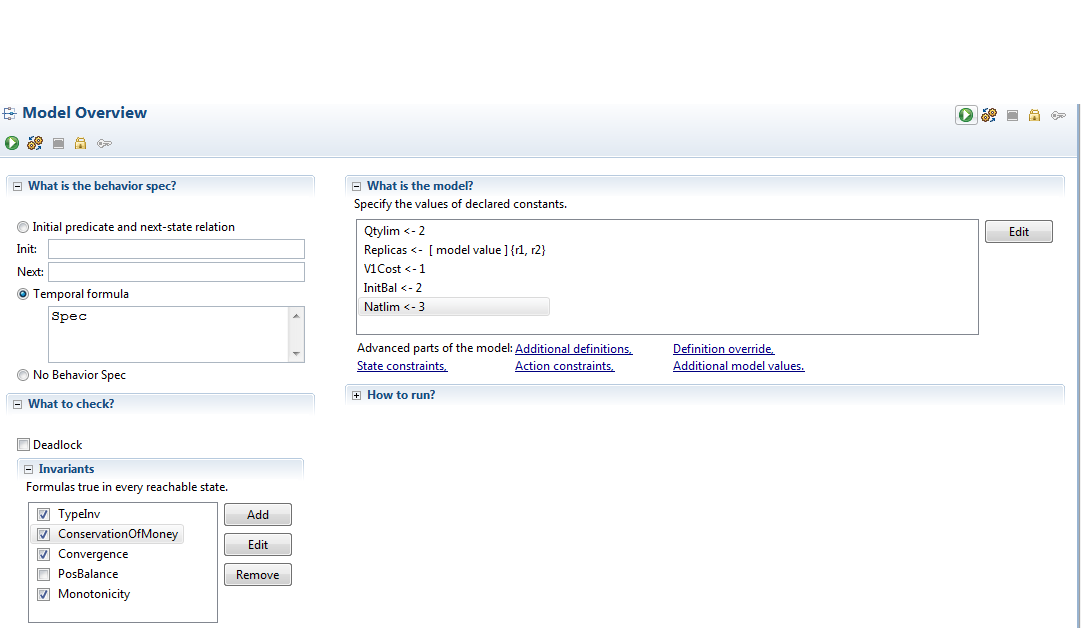
\includegraphics[scale=1.0]{TLA/latexDocs/walletv4.dvi}

\subsubsection{Wallet use case using Integers}
The balance and the counts of the vouchers in the wallets are integers instead of PN-Counters. When two copies of a wallet account are merged the maximum of the balances of the wallets is taken so the balance is generous for the player. When merging the total count of vouchers, the amount of vouchers is added in the two copies. As expected, when it is tested in TLC some money is lost, i.e. the total money spend is more than the money reduced from the balance. The TLA+ representation for this particular example is presented bellow.

%\verbinput{TLA/walletNat.tla}
%\tlatex
\@x{}\moduleLeftDash\@xx{ {\MODULE} walletNat}\moduleRightDash\@xx{}%
\@x{ {\EXTENDS} Integers ,\, TLC ,\, Naturals}%
\@x{ {\VARIABLE} wallets}%
\@x{ {\CONSTANTS} Replicas ,\, V1Cost ,\, InitBal ,\, Natlim ,\, Qtylim}%
\@pvspace{8.0pt}%
\@x{}\midbar\@xx{}%
\@pvspace{8.0pt}%
\@x{ Wallet \.{\defeq} [ balance \.{:} Int ,\,}%
\@x{\@s{51.25} v1cnt \.{:} Int ,\,}%
\@x{\@s{51.25} vecclc \.{:} [ Replicas \.{\rightarrow} Nat ] ]}%
\@pvspace{8.0pt}%
 \@x{ TypeInv \.{\defeq} \.{\land} wallets \.{\in} [ Replicas \.{\rightarrow}
 Wallet ]}%
\@pvspace{8.0pt}%
 \@x{ Init \.{\defeq}\@s{4.1} \.{\land} wallets \.{=} [ r \.{\in} Replicas
 \.{\mapsto} [ balance \.{\mapsto} InitBal ,\,}%
\@x{\@s{170.42} v1cnt \.{\mapsto} 0 ,\,}%
\@x{\@s{170.42} vecclc \.{\mapsto} [ r2 \.{\in} Replicas \.{\mapsto} 0 ] ] ]}%
\@x{\@s{29.11} \.{\land} Print ( wallets ,\, {\TRUE} )}%
\@pvspace{8.0pt}%
\@x{ BuyV1 ( rep ,\, qty ) \.{\defeq}}%
\@x{\@s{16.4} \.{\LET} wr \.{\defeq} wallets [ rep ]}%
 \@x{\@s{36.79} new\_vc\@s{2.17} \.{\defeq} [ wr . vecclc {\EXCEPT} {\bang} [
 rep ] \.{=} wr . vecclc [ rep ] \.{+} 1 ]}%
 \@x{\@s{36.79} new\_wr \.{\defeq} [ balance \.{\mapsto} wr . balance \.{-}
 qty \.{*} V1Cost ,\,}%
\@x{\@s{92.84} v1cnt \.{\mapsto} wr . v1cnt \.{+} qty ,\,}%
\@x{\@s{92.84} vecclc \.{\mapsto} new\_vc ]}%
\@x{\@s{16.4} \.{\IN} \.{\land} wr . balance \.{\geq} qty \.{*} V1Cost}%
\@x{\@s{36.79} \.{\land} wr . v1cnt \.{+} qty \.{\leq} Natlim}%
\@x{\@s{36.79} \.{\land} wr . vecclc [ rep ] \.{+} 1 \.{\leq} Natlim}%
 \@x{\@s{36.79} \.{\land} wallets \.{'}\@s{18.09} \.{=} [ wallets {\EXCEPT}
 {\bang} [ rep ] \.{=} new\_wr ]}%
\@pvspace{8.0pt}%
 \@x{ Max ( n1 ,\, n2 ) \.{\defeq} {\IF} n1 \.{\geq} n2 \.{\THEN} n1 \.{\ELSE}
 n2}%
\@pvspace{8.0pt}%
\@x{ Merge ( r1 ,\, r2 ) \.{\defeq}}%
\@x{\@s{16.4} \.{\LET} wr1 \.{\defeq} wallets [ r1 ]}%
\@x{\@s{36.79} wr2 \.{\defeq} wallets [ r2 ]}%
 \@x{\@s{36.79} new\_vc\@s{2.95} \.{\defeq} [ r \.{\in} Replicas \.{\mapsto}
 Max ( wr1 . vecclc [ r ] ,\, wr2 . vecclc [ r ] ) ]}%
 \@x{\@s{36.79} new\_w1 \.{\defeq} [ balance \.{\mapsto} Max ( wr1 . balance
 ,\, wr2 . balance ) ,\,}%
\@x{\@s{93.62} v1cnt \.{\mapsto} Max ( wr1 . v1cnt ,\, wr2 . v1cnt ) ,\,}%
\@y{\@s{0}%
 alternative formulation: \ensuremath{wr1.v1cnt\.{+}wr2.v1cnt
}}%
\@xx{}%
\@x{\@s{93.62} vecclc \.{\mapsto} new\_vc ]}%
\@pvspace{8.0pt}%
 \@x{\@s{16.4} \.{\IN} \.{\land} \E\, r \.{\in} Replicas \.{:} wr1 . vecclc [
 r ] \.{<} wr2 . vecclc [ r ]}%
 \@x{\@s{36.79} \.{\land} wallets \.{'} \.{=} [ wallets {\EXCEPT} {\bang} [ r1
 ] \.{=} new\_w1 ]}%
\@pvspace{16.0pt}%
 \@x{ ConservationOfMoney \.{\defeq} \A\, r \.{\in} Replicas \.{:} ( InitBal
 \.{-} wallets [ r ] . balance ) \.{\geq} wallets [ r ] . v1cnt \.{*} V1Cost}%
\@pvspace{8.0pt}%
 \@x{ FinalState ( vc ) \.{\defeq} \A\, r \.{\in} Replicas \.{:} vc [ r ]
 \.{=} Natlim}%
 \@x{ EqualStates ( st1 ,\, st2 ) \.{\defeq} st1 . balance \.{=} st2 . balance
 \.{\land} st1 . v1cnt \.{=} st2 . v1cnt}%
 \@x{ Convergence \.{\defeq} \A\, r1 \.{\in} Replicas ,\, r2 \.{\in} Replicas
 \.{:}}%
 \@x{\@s{32.8} FinalState ( wallets [ r1 ] . vecclc ) \.{\land} FinalState (
 wallets [ r2 ] . vecclc ) \.{\implies}}%
\@x{\@s{65.6} EqualStates ( wallets [ r1 ] ,\, wallets [ r2 ] )}%
\@pvspace{8.0pt}%
 \@x{ Next \.{\defeq} \E\, r1 \.{\in} Replicas ,\, r2 \.{\in} Replicas ,\, qty
 \.{\in} 1 \.{\dotdot} Qtylim \.{:} ( BuyV1 ( r1 ,\, qty ) \.{\lor} Merge (
 r1 ,\, r2 ) )}%
\@pvspace{8.0pt}%
 \@x{ Spec\@s{1.46} \.{\defeq} Init \.{\land} {\Box} [ Next ]_{ {\langle}
 wallets {\rangle}}}%
\@pvspace{8.0pt}%
 \@x{ {\THEOREM} Spec \.{\implies} TypeInv \.{\land} ConservationOfMoney
 \.{\land} Convergence}%
\@x{}\bottombar\@xx{}%

\subsubsection{Wallet use case using No Atomic Operations}
In here it is presented the scenario in which buying some vouchers is not an atomic operation. For this model, it is defined two operators so that PN-Counters, which keep the balance and voucher counts, could be merged separately. As expected again, some money is lost and some properties are not satisfied. The TLA+ representation for this particular example is presented bellow.

%\verbinput{TLA/walletWOTx.tla}
%\batchmode %% Suppresses most terminal output.
\documentclass{article}
\setlength{\textwidth}{360pt}
\setlength{\textheight}{541pt}
\usepackage{latexsym}
\usepackage{ifthen}
% \usepackage{color}
%%%%%%%%%%%%%%%%%%%%%%%%%%%%%%%%%%%%%%%%%%%%%%%%%%%%%%%%%%%%%%%%%%%%%%%%%%%%%
% SWITCHES                                                                  %
%%%%%%%%%%%%%%%%%%%%%%%%%%%%%%%%%%%%%%%%%%%%%%%%%%%%%%%%%%%%%%%%%%%%%%%%%%%%%
\newboolean{shading} 
\setboolean{shading}{false}
\makeatletter
 %% this is needed only when inserted into the file, not when
 %% used as a package file.
%%%%%%%%%%%%%%%%%%%%%%%%%%%%%%%%%%%%%%%%%%%%%%%%%%%%%%%%%%%%%%%%%%%%%%%%%%%%%
%                                                                           %
% DEFINITIONS OF SYMBOL-PRODUCING COMMANDS                                  %
%                                                                           %
%    TLA+      LaTeX                                                        %
%    symbol    command                                                      %
%    ------    -------                                                      %
%    =>        \implies                                                     %
%    <:        \ltcolon                                                     %
%    :>        \colongt                                                     %
%    ==        \defeq                                                       %
%    ..        \dotdot                                                      %
%    ::        \coloncolon                                                  %
%    =|        \eqdash                                                      %
%    ++        \pp                                                          %
%    --        \mm                                                          %
%    **        \stst                                                        %
%    //        \slsl                                                        %
%    ^         \ct                                                          %
%    \A        \A                                                           %
%    \E        \E                                                           %
%    \AA       \AA                                                          %
%    \EE       \EE                                                          %
%%%%%%%%%%%%%%%%%%%%%%%%%%%%%%%%%%%%%%%%%%%%%%%%%%%%%%%%%%%%%%%%%%%%%%%%%%%%%
\newlength{\symlength}
\newcommand{\implies}{\Rightarrow}
\newcommand{\ltcolon}{\mathrel{<\!\!\mbox{:}}}
\newcommand{\colongt}{\mathrel{\!\mbox{:}\!\!>}}
\newcommand{\defeq}{\;\mathrel{\smash   %% keep this symbol from being too tall
    {{\stackrel{\scriptscriptstyle\Delta}{=}}}}\;}
\newcommand{\dotdot}{\mathrel{\ldotp\ldotp}}
\newcommand{\coloncolon}{\mathrel{::\;}}
\newcommand{\eqdash}{\mathrel = \joinrel \hspace{-.28em}|}
\newcommand{\pp}{\mathbin{++}}
\newcommand{\mm}{\mathbin{--}}
\newcommand{\stst}{*\!*}
\newcommand{\slsl}{/\!/}
\newcommand{\ct}{\hat{\hspace{.4em}}}
\newcommand{\A}{\forall}
\newcommand{\E}{\exists}
\renewcommand{\AA}{\makebox{$\raisebox{.05em}{\makebox[0pt][l]{%
   $\forall\hspace{-.517em}\forall\hspace{-.517em}\forall$}}%
   \forall\hspace{-.517em}\forall \hspace{-.517em}\forall\,$}}
\newcommand{\EE}{\makebox{$\raisebox{.05em}{\makebox[0pt][l]{%
   $\exists\hspace{-.517em}\exists\hspace{-.517em}\exists$}}%
   \exists\hspace{-.517em}\exists\hspace{-.517em}\exists\,$}}
\newcommand{\whileop}{\.{\stackrel
  {\mbox{\raisebox{-.3em}[0pt][0pt]{$\scriptscriptstyle+\;\,$}}}%
  {-\hspace{-.16em}\triangleright}}}

% Commands are defined to produce the upper-case keywords.
% Note that some have space after them.
\newcommand{\ASSUME}{\textsc{assume }}
\newcommand{\ASSUMPTION}{\textsc{assumption }}
\newcommand{\AXIOM}{\textsc{axiom }}
\newcommand{\BOOLEAN}{\textsc{boolean }}
\newcommand{\CASE}{\textsc{case }}
\newcommand{\CONSTANT}{\textsc{constant }}
\newcommand{\CONSTANTS}{\textsc{constants }}
\newcommand{\ELSE}{\settowidth{\symlength}{\THEN}%
   \makebox[\symlength][l]{\textsc{ else}}}
\newcommand{\EXCEPT}{\textsc{ except }}
\newcommand{\EXTENDS}{\textsc{extends }}
\newcommand{\FALSE}{\textsc{false}}
\newcommand{\IF}{\textsc{if }}
\newcommand{\IN}{\settowidth{\symlength}{\LET}%
   \makebox[\symlength][l]{\textsc{in}}}
\newcommand{\INSTANCE}{\textsc{instance }}
\newcommand{\LET}{\textsc{let }}
\newcommand{\LOCAL}{\textsc{local }}
\newcommand{\MODULE}{\textsc{module }}
\newcommand{\OTHER}{\textsc{other }}
\newcommand{\STRING}{\textsc{string}}
\newcommand{\THEN}{\textsc{ then }}
\newcommand{\THEOREM}{\textsc{theorem }}
\newcommand{\LEMMA}{\textsc{lemma }}
\newcommand{\PROPOSITION}{\textsc{proposition }}
\newcommand{\COROLLARY}{\textsc{corollary }}
\newcommand{\TRUE}{\textsc{true}}
\newcommand{\VARIABLE}{\textsc{variable }}
\newcommand{\VARIABLES}{\textsc{variables }}
\newcommand{\WITH}{\textsc{ with }}
\newcommand{\WF}{\textrm{WF}}
\newcommand{\SF}{\textrm{SF}}
\newcommand{\CHOOSE}{\textsc{choose }}
\newcommand{\ENABLED}{\textsc{enabled }}
\newcommand{\UNCHANGED}{\textsc{unchanged }}
\newcommand{\SUBSET}{\textsc{subset }}
\newcommand{\UNION}{\textsc{union }}
\newcommand{\DOMAIN}{\textsc{domain }}
% Added for tla2tex
\newcommand{\BY}{\textsc{by }}
\newcommand{\OBVIOUS}{\textsc{obvious }}
\newcommand{\HAVE}{\textsc{have }}
\newcommand{\QED}{\textsc{qed }}
\newcommand{\TAKE}{\textsc{take }}
\newcommand{\DEF}{\textsc{ def }}
\newcommand{\HIDE}{\textsc{hide }}
\newcommand{\RECURSIVE}{\textsc{recursive }}
\newcommand{\USE}{\textsc{use }}
\newcommand{\DEFINE}{\textsc{define }}
\newcommand{\PROOF}{\textsc{proof }}
\newcommand{\WITNESS}{\textsc{witness }}
\newcommand{\PICK}{\textsc{pick }}
\newcommand{\DEFS}{\textsc{defs }}
\newcommand{\PROVE}{\settowidth{\symlength}{\ASSUME}%
   \makebox[\symlength][l]{\textsc{prove}}\@s{-4.1}}%
  %% The \@s{-4.1) is a kludge added on 24 Oct 2009 [happy birthday, Ellen]
  %% so the correct alignment occurs if the user types
  %%   ASSUME X
  %%   PROVE  Y
  %% because it cancels the extra 4.1 pts added because of the 
  %% extra space after the PROVE.  This seems to works OK.
  %% However, the 4.1 equals Parameters.LaTeXLeftSpace(1) and
  %% should be changed if that method ever changes.
\newcommand{\SUFFICES}{\textsc{suffices }}
\newcommand{\NEW}{\textsc{new }}
\newcommand{\LAMBDA}{\textsc{lambda }}
\newcommand{\STATE}{\textsc{state }}
\newcommand{\ACTION}{\textsc{action }}
\newcommand{\TEMPORAL}{\textsc{temporal }}
\newcommand{\ONLY}{\textsc{only }}              %% added by LL on 2 Oct 2009
\newcommand{\OMITTED}{\textsc{omitted }}        %% added by LL on 31 Oct 2009
\newcommand{\@pfstepnum}[2]{\ensuremath{\langle#1\rangle}\textrm{#2}}
\newcommand{\bang}{\@s{1}\mbox{\small !}\@s{1}}
%% We should format || differently in PlusCal code than in TLA+ formulas.
\newcommand{\p@barbar}{\ifpcalsymbols
   \,\,\rule[-.25em]{.075em}{1em}\hspace*{.2em}\rule[-.25em]{.075em}{1em}\,\,%
   \else \,||\,\fi}
%% PlusCal keywords
\newcommand{\p@fair}{\textbf{fair }}
\newcommand{\p@semicolon}{\textbf{\,; }}
\newcommand{\p@algorithm}{\textbf{algorithm }}
\newcommand{\p@mmfair}{\textbf{-{}-fair }}
\newcommand{\p@mmalgorithm}{\textbf{-{}-algorithm }}
\newcommand{\p@assert}{\textbf{assert }}
\newcommand{\p@await}{\textbf{await }}
\newcommand{\p@begin}{\textbf{begin }}
\newcommand{\p@end}{\textbf{end }}
\newcommand{\p@call}{\textbf{call }}
\newcommand{\p@define}{\textbf{define }}
\newcommand{\p@do}{\textbf{ do }}
\newcommand{\p@either}{\textbf{either }}
\newcommand{\p@or}{\textbf{or }}
\newcommand{\p@goto}{\textbf{goto }}
\newcommand{\p@if}{\textbf{if }}
\newcommand{\p@then}{\,\,\textbf{then }}
\newcommand{\p@else}{\ifcsyntax \textbf{else } \else \,\,\textbf{else }\fi}
\newcommand{\p@elsif}{\,\,\textbf{elsif }}
\newcommand{\p@macro}{\textbf{macro }}
\newcommand{\p@print}{\textbf{print }}
\newcommand{\p@procedure}{\textbf{procedure }}
\newcommand{\p@process}{\textbf{process }}
\newcommand{\p@return}{\textbf{return}}
\newcommand{\p@skip}{\textbf{skip}}
\newcommand{\p@variable}{\textbf{variable }}
\newcommand{\p@variables}{\textbf{variables }}
\newcommand{\p@while}{\textbf{while }}
\newcommand{\p@when}{\textbf{when }}
\newcommand{\p@with}{\textbf{with }}
\newcommand{\p@lparen}{\textbf{(\,\,}}
\newcommand{\p@rparen}{\textbf{\,\,) }}   
\newcommand{\p@lbrace}{\textbf{\{\,\,}}   
\newcommand{\p@rbrace}{\textbf{\,\,\} }}

%%%%%%%%%%%%%%%%%%%%%%%%%%%%%%%%%%%%%%%%%%%%%%%%%%%%%%%%%
% REDEFINE STANDARD COMMANDS TO MAKE THEM FORMAT BETTER %
%                                                       %
% We redefine \in and \notin                            %
%%%%%%%%%%%%%%%%%%%%%%%%%%%%%%%%%%%%%%%%%%%%%%%%%%%%%%%%%
\renewcommand{\_}{\rule{.4em}{.06em}\hspace{.05em}}
\newlength{\equalswidth}
\let\oldin=\in
\let\oldnotin=\notin
\renewcommand{\in}{%
   {\settowidth{\equalswidth}{$\.{=}$}\makebox[\equalswidth][c]{$\oldin$}}}
\renewcommand{\notin}{%
   {\settowidth{\equalswidth}{$\.{=}$}\makebox[\equalswidth]{$\oldnotin$}}}


%%%%%%%%%%%%%%%%%%%%%%%%%%%%%%%%%%%%%%%%%%%%%%%%%%%%
%                                                  %
% HORIZONTAL BARS:                                 %
%                                                  %
%   \moduleLeftDash    |~~~~~~~~~~                 %
%   \moduleRightDash    ~~~~~~~~~~|                %
%   \midbar            |----------|                %
%   \bottombar         |__________|                %
%%%%%%%%%%%%%%%%%%%%%%%%%%%%%%%%%%%%%%%%%%%%%%%%%%%%
\newlength{\charwidth}\settowidth{\charwidth}{{\small\tt M}}
\newlength{\boxrulewd}\setlength{\boxrulewd}{.4pt}
\newlength{\boxlineht}\setlength{\boxlineht}{.5\baselineskip}
\newcommand{\boxsep}{\charwidth}
\newlength{\boxruleht}\setlength{\boxruleht}{.5ex}
\newlength{\boxruledp}\setlength{\boxruledp}{-\boxruleht}
\addtolength{\boxruledp}{\boxrulewd}
\newcommand{\boxrule}{\leaders\hrule height \boxruleht depth \boxruledp
                      \hfill\mbox{}}
\newcommand{\@computerule}{%
  \setlength{\boxruleht}{.5ex}%
  \setlength{\boxruledp}{-\boxruleht}%
  \addtolength{\boxruledp}{\boxrulewd}}

\newcommand{\bottombar}{\hspace{-\boxsep}%
  \raisebox{-\boxrulewd}[0pt][0pt]{\rule[.5ex]{\boxrulewd}{\boxlineht}}%
  \boxrule
  \raisebox{-\boxrulewd}[0pt][0pt]{%
      \rule[.5ex]{\boxrulewd}{\boxlineht}}\hspace{-\boxsep}\vspace{0pt}}

\newcommand{\moduleLeftDash}%
   {\hspace*{-\boxsep}%
     \raisebox{-\boxlineht}[0pt][0pt]{\rule[.5ex]{\boxrulewd
               }{\boxlineht}}%
    \boxrule\hspace*{.4em }}

\newcommand{\moduleRightDash}%
    {\hspace*{.4em}\boxrule
    \raisebox{-\boxlineht}[0pt][0pt]{\rule[.5ex]{\boxrulewd
               }{\boxlineht}}\hspace{-\boxsep}}%\vspace{.2em}

\newcommand{\midbar}{\hspace{-\boxsep}\raisebox{-.5\boxlineht}[0pt][0pt]{%
   \rule[.5ex]{\boxrulewd}{\boxlineht}}\boxrule\raisebox{-.5\boxlineht%
   }[0pt][0pt]{\rule[.5ex]{\boxrulewd}{\boxlineht}}\hspace{-\boxsep}}

%%%%%%%%%%%%%%%%%%%%%%%%%%%%%%%%%%%%%%%%%%%%%%%%%%%%%%%%%%%%%%%%%%%%%%%%%%%%%
% FORMATING COMMANDS                                                        %
%%%%%%%%%%%%%%%%%%%%%%%%%%%%%%%%%%%%%%%%%%%%%%%%%%%%%%%%%%%%%%%%%%%%%%%%%%%%%

%%%%%%%%%%%%%%%%%%%%%%%%%%%%%%%%%%%%%%%%%%%%%%%%%%%%%%%%%%%%%%%%%%%%%%%%%%%%%
% PLUSCAL SHADING                                                           %
%%%%%%%%%%%%%%%%%%%%%%%%%%%%%%%%%%%%%%%%%%%%%%%%%%%%%%%%%%%%%%%%%%%%%%%%%%%%%

% The TeX pcalshading switch is set on to cause PlusCal shading to be
% performed.  This changes the behavior of the following commands and
% environments to cause full-width shading to be performed on all lines.
% 
%   \tstrut \@x cpar mcom \@pvspace
% 
% The TeX pcalsymbols switch is turned on when typesetting a PlusCal algorithm,
% whether or not shading is being performed.  It causes symbols (other than
% parentheses and braces and PlusCal-only keywords) that should be typeset
% differently depending on whether they are in an algorithm to be typeset
% appropriately.  Currently, the only such symbol is "||".
%
% The TeX csyntax switch is turned on when typesetting a PlusCal algorithm in
% c-syntax.  This allows symbols to be format differently in the two syntaxes.
% The "else" keyword is the only one that is.

\newif\ifpcalshading \pcalshadingfalse
\newif\ifpcalsymbols \pcalsymbolsfalse
\newif\ifcsyntax     \csyntaxtrue

% The \@pvspace command makes a vertical space.  It uses \vspace
% except with \ifpcalshading, in which case it sets \pvcalvspace
% and the space is added by a following \@x command.
%
\newlength{\pcalvspace}\setlength{\pcalvspace}{0pt}%
\newcommand{\@pvspace}[1]{%
  \ifpcalshading
     \par\global\setlength{\pcalvspace}{#1}%
  \else
     \par\vspace{#1}%
  \fi
}

% The lcom environment was changed to set \lcomindent equal to
% the indentation it produces.  This length is used by the
% cpar environment to make shading extend for the full width
% of the line.  This assumes that lcom environments are not
% nested.  I hope TLATeX does not nest them.
%
\newlength{\lcomindent}%
\setlength{\lcomindent}{0pt}%

%\tstrut: A strut to produce inter-paragraph space in a comment.
%\rstrut: A strut to extend the bottom of a one-line comment so
%         there's no break in the shading between comments on 
%         successive lines.
\newcommand\tstrut%
  {\raisebox{\vshadelen}{\raisebox{-.25em}{\rule{0pt}{1.15em}}}%
   \global\setlength{\vshadelen}{0pt}}
\newcommand\rstrut{\raisebox{-.25em}{\rule{0pt}{1.15em}}%
 \global\setlength{\vshadelen}{0pt}}


% \.{op} formats operator op in math mode with empty boxes on either side.
% Used because TeX otherwise vary the amount of space it leaves around op.
\renewcommand{\.}[1]{\ensuremath{\mbox{}#1\mbox{}}}

% \@s{n} produces an n-point space
\newcommand{\@s}[1]{\hspace{#1pt}}           

% \@x{txt} starts a specification line in the beginning with txt
% in the final LaTeX source.
\newlength{\@xlen}
\newcommand\xtstrut%
  {\setlength{\@xlen}{1.05em}%
   \addtolength{\@xlen}{\pcalvspace}%
    \raisebox{\vshadelen}{\raisebox{-.25em}{\rule{0pt}{\@xlen}}}%
   \global\setlength{\vshadelen}{0pt}%
   \global\setlength{\pcalvspace}{0pt}}

\newcommand{\@x}[1]{\par
  \ifpcalshading
  \makebox[0pt][l]{\shadebox{\xtstrut\hspace*{\textwidth}}}%
  \fi
  \mbox{$\mbox{}#1\mbox{}$}}  

% \@xx{txt} continues a specification line with the text txt.
\newcommand{\@xx}[1]{\mbox{$\mbox{}#1\mbox{}$}}  

% \@y{cmt} produces a one-line comment.
\newcommand{\@y}[1]{\mbox{\footnotesize\hspace{.65em}%
  \ifthenelse{\boolean{shading}}{%
      \shadebox{#1\hspace{-\the\lastskip}\rstrut}}%
               {#1\hspace{-\the\lastskip}\rstrut}}}

% \@z{cmt} produces a zero-width one-line comment.
\newcommand{\@z}[1]{\makebox[0pt][l]{\footnotesize
  \ifthenelse{\boolean{shading}}{%
      \shadebox{#1\hspace{-\the\lastskip}\rstrut}}%
               {#1\hspace{-\the\lastskip}\rstrut}}}


% \@w{str} produces the TLA+ string "str".
\newcommand{\@w}[1]{\textsf{``{#1}''}}             


%%%%%%%%%%%%%%%%%%%%%%%%%%%%%%%%%%%%%%%%%%%%%%%%%%%%%%%%%%%%%%%%%%%%%%%%%%%%%
% SHADING                                                                   %
%%%%%%%%%%%%%%%%%%%%%%%%%%%%%%%%%%%%%%%%%%%%%%%%%%%%%%%%%%%%%%%%%%%%%%%%%%%%%
\def\graymargin{1}
  % The number of points of margin in the shaded box.

% \definecolor{boxshade}{gray}{.85}
% Defines the darkness of the shading: 1 = white, 0 = black
% Added by TLATeX only if needed.

% \shadebox{txt} puts txt in a shaded box.
\newlength{\templena}
\newlength{\templenb}
\newsavebox{\tempboxa}
\newcommand{\shadebox}[1]{{\setlength{\fboxsep}{\graymargin pt}%
     \savebox{\tempboxa}{#1}%
     \settoheight{\templena}{\usebox{\tempboxa}}%
     \settodepth{\templenb}{\usebox{\tempboxa}}%
     \hspace*{-\fboxsep}\raisebox{0pt}[\templena][\templenb]%
        {\colorbox{boxshade}{\usebox{\tempboxa}}}\hspace*{-\fboxsep}}}

% \vshade{n} makes an n-point inter-paragraph space, with
%  shading if the `shading' flag is true.
\newlength{\vshadelen}
\setlength{\vshadelen}{0pt}
\newcommand{\vshade}[1]{\ifthenelse{\boolean{shading}}%
   {\global\setlength{\vshadelen}{#1pt}}%
   {\vspace{#1pt}}}

\newlength{\boxwidth}
\newlength{\multicommentdepth}

%%%%%%%%%%%%%%%%%%%%%%%%%%%%%%%%%%%%%%%%%%%%%%%%%%%%%%%%%%%%%%%%%%%%%%%%%%%%%
% THE cpar ENVIRONMENT                                                      %
% ^^^^^^^^^^^^^^^^^^^^                                                      %
% The LaTeX input                                                           %
%                                                                           %
%   \begin{cpar}{pop}{nest}{isLabel}{d}{e}{arg6}                            %
%     XXXXXXXXXXXXXXX                                                       %
%     XXXXXXXXXXXXXXX                                                       %
%     XXXXXXXXXXXXXXX                                                       %
%   \end{cpar}                                                              %
%                                                                           %
% produces one of two possible results.  If isLabel is the letter "T",      %
% it produces the following, where [label] is the result of typesetting     %
% arg6 in an LR box, and d is is a number representing a distance in        %
% points.                                                                   %
%                                                                           %
%   prevailing |<-- d -->[label]<- e ->XXXXXXXXXXXXXXX                      %
%         left |                       XXXXXXXXXXXXXXX                      %
%       margin |                       XXXXXXXXXXXXXXX                      %
%                                                                           %
% If isLabel is the letter "F", then it produces                            %
%                                                                           %
%   prevailing |<-- d -->XXXXXXXXXXXXXXXXXXXXXXX                            %
%         left |         <- e ->XXXXXXXXXXXXXXXX                            %
%       margin |                XXXXXXXXXXXXXXXX                            %
%                                                                           %
% where d and e are numbers representing distances in points.               %
%                                                                           %
% The prevailing left margin is the one in effect before the most recent    %
% pop (argument 1) cpar environments with "T" as the nest argument, where   %
% pop is a number \geq 0.                                                   %
%                                                                           %
% If the nest argument is the letter "T", then the prevailing left          %
% margin is moved to the left of the second (and following) lines of        %
% X's.  Otherwise, the prevailing left margin is left unchanged.            %
%                                                                           %
% An \unnest{n} command moves the prevailing left margin to where it was    %
% before the most recent n cpar environments with "T" as the nesting        %
% argument.                                                                 %
%                                                                           %
% The environment leaves no vertical space above or below it, or between    %
% its paragraphs.  (TLATeX inserts the proper amount of vertical space.)    %
%%%%%%%%%%%%%%%%%%%%%%%%%%%%%%%%%%%%%%%%%%%%%%%%%%%%%%%%%%%%%%%%%%%%%%%%%%%%%

\newcounter{pardepth}
\setcounter{pardepth}{0}

% \setgmargin{txt} defines \gmarginN to be txt, where N is \roman{pardepth}.
% \thegmargin equals \gmarginN, where N is \roman{pardepth}.
\newcommand{\setgmargin}[1]{%
  \expandafter\xdef\csname gmargin\roman{pardepth}\endcsname{#1}}
\newcommand{\thegmargin}{\csname gmargin\roman{pardepth}\endcsname}
\newcommand{\gmargin}{0pt}

\newsavebox{\tempsbox}

\newlength{\@cparht}
\newlength{\@cpardp}
\newenvironment{cpar}[6]{%
  \addtocounter{pardepth}{-#1}%
  \ifthenelse{\boolean{shading}}{\par\begin{lrbox}{\tempsbox}%
                                 \begin{minipage}[t]{\linewidth}}{}%
  \begin{list}{}{%
     \edef\temp{\thegmargin}
     \ifthenelse{\equal{#3}{T}}%
       {\settowidth{\leftmargin}{\hspace{\temp}\footnotesize #6\hspace{#5pt}}%
        \addtolength{\leftmargin}{#4pt}}%
       {\setlength{\leftmargin}{#4pt}%
        \addtolength{\leftmargin}{#5pt}%
        \addtolength{\leftmargin}{\temp}%
        \setlength{\itemindent}{-#5pt}}%
      \ifthenelse{\equal{#2}{T}}{\addtocounter{pardepth}{1}%
                                 \setgmargin{\the\leftmargin}}{}%
      \setlength{\labelwidth}{0pt}%
      \setlength{\labelsep}{0pt}%
      \setlength{\itemindent}{-\leftmargin}%
      \setlength{\topsep}{0pt}%
      \setlength{\parsep}{0pt}%
      \setlength{\partopsep}{0pt}%
      \setlength{\parskip}{0pt}%
      \setlength{\itemsep}{0pt}
      \setlength{\itemindent}{#4pt}%
      \addtolength{\itemindent}{-\leftmargin}}%
   \ifthenelse{\equal{#3}{T}}%
      {\item[\tstrut\footnotesize \hspace{\temp}{#6}\hspace{#5pt}]
        }%
      {\item[\tstrut\hspace{\temp}]%
         }%
   \footnotesize}
 {\hspace{-\the\lastskip}\tstrut
 \end{list}%
  \ifthenelse{\boolean{shading}}%
          {\end{minipage}%
           \end{lrbox}%
           \ifpcalshading
             \setlength{\@cparht}{\ht\tempsbox}%
             \setlength{\@cpardp}{\dp\tempsbox}%
             \addtolength{\@cparht}{.15em}%
             \addtolength{\@cpardp}{.2em}%
             \addtolength{\@cparht}{\@cpardp}%
            % I don't know what's going on here.  I want to add a
            % \pcalvspace high shaded line, but I don't know how to
            % do it.  A little trial and error shows that the following
            % does a reasonable job approximating that, eliminating
            % the line if \pcalvspace is small.
            \addtolength{\@cparht}{\pcalvspace}%
             \ifdim \pcalvspace > .8em
               \addtolength{\pcalvspace}{-.2em}%
               \hspace*{-\lcomindent}%
               \shadebox{\rule{0pt}{\pcalvspace}\hspace*{\textwidth}}\par
               \global\setlength{\pcalvspace}{0pt}%
               \fi
             \hspace*{-\lcomindent}%
             \makebox[0pt][l]{\raisebox{-\@cpardp}[0pt][0pt]{%
                 \shadebox{\rule{0pt}{\@cparht}\hspace*{\textwidth}}}}%
             \hspace*{\lcomindent}\usebox{\tempsbox}%
             \par
           \else
             \shadebox{\usebox{\tempsbox}}\par
           \fi}%
           {}%
  }

%%%%%%%%%%%%%%%%%%%%%%%%%%%%%%%%%%%%%%%%%%%%%%%%%%%%%%%%%%%%%%%%%%%%%%%%%%%%%%
% THE ppar ENVIRONMENT                                                       %
% ^^^^^^^^^^^^^^^^^^^^                                                       %
% The environment                                                            %
%                                                                            %
%   \begin{ppar} ... \end{ppar}                                              %
%                                                                            %
% is equivalent to                                                           %
%                                                                            %
%   \begin{cpar}{0}{F}{F}{0}{0}{} ... \end{cpar}                             %
%                                                                            %
% The environment is put around each line of the output for a PlusCal        %
% algorithm.                                                                 %
%%%%%%%%%%%%%%%%%%%%%%%%%%%%%%%%%%%%%%%%%%%%%%%%%%%%%%%%%%%%%%%%%%%%%%%%%%%%%%
%\newenvironment{ppar}{%
%  \ifthenelse{\boolean{shading}}{\par\begin{lrbox}{\tempsbox}%
%                                 \begin{minipage}[t]{\linewidth}}{}%
%  \begin{list}{}{%
%     \edef\temp{\thegmargin}
%        \setlength{\leftmargin}{0pt}%
%        \addtolength{\leftmargin}{\temp}%
%        \setlength{\itemindent}{0pt}%
%      \setlength{\labelwidth}{0pt}%
%      \setlength{\labelsep}{0pt}%
%      \setlength{\itemindent}{-\leftmargin}%
%      \setlength{\topsep}{0pt}%
%      \setlength{\parsep}{0pt}%
%      \setlength{\partopsep}{0pt}%
%      \setlength{\parskip}{0pt}%
%      \setlength{\itemsep}{0pt}
%      \setlength{\itemindent}{0pt}%
%      \addtolength{\itemindent}{-\leftmargin}}%
%      \item[\tstrut\hspace{\temp}]}%
% {\hspace{-\the\lastskip}\tstrut
% \end{list}%
%  \ifthenelse{\boolean{shading}}{\end{minipage}  
%                                 \end{lrbox}%
%                                 \shadebox{\usebox{\tempsbox}}\par}{}%
%  }

 %%% TESTING
 \newcommand{\xtest}[1]{\par
 \makebox[0pt][l]{\shadebox{\xtstrut\hspace*{\textwidth}}}%
 \mbox{$\mbox{}#1\mbox{}$}} 

% \newcommand{\xxtest}[1]{\par
% \makebox[0pt][l]{\shadebox{\xtstrut{#1}\hspace*{\textwidth}}}%
% \mbox{$\mbox{}#1\mbox{}$}} 

%\newlength{\pcalvspace}
%\setlength{\pcalvspace}{0pt}
% \newlength{\xxtestlen}
% \setlength{\xxtestlen}{0pt}
% \newcommand\xtstrut%
%   {\setlength{\xxtestlen}{1.15em}%
%    \addtolength{\xxtestlen}{\pcalvspace}%
%     \raisebox{\vshadelen}{\raisebox{-.25em}{\rule{0pt}{\xxtestlen}}}%
%    \global\setlength{\vshadelen}{0pt}%
%    \global\setlength{\pcalvspace}{0pt}}
   
   %%%% TESTING
   
   %% The xcpar environment
   %%  Note: overloaded use of \pcalvspace for testing.
   %%
%   \newlength{\xcparht}%
%   \newlength{\xcpardp}%
   
%   \newenvironment{xcpar}[6]{%
%  \addtocounter{pardepth}{-#1}%
%  \ifthenelse{\boolean{shading}}{\par\begin{lrbox}{\tempsbox}%
%                                 \begin{minipage}[t]{\linewidth}}{}%
%  \begin{list}{}{%
%     \edef\temp{\thegmargin}%
%     \ifthenelse{\equal{#3}{T}}%
%       {\settowidth{\leftmargin}{\hspace{\temp}\footnotesize #6\hspace{#5pt}}%
%        \addtolength{\leftmargin}{#4pt}}%
%       {\setlength{\leftmargin}{#4pt}%
%        \addtolength{\leftmargin}{#5pt}%
%        \addtolength{\leftmargin}{\temp}%
%        \setlength{\itemindent}{-#5pt}}%
%      \ifthenelse{\equal{#2}{T}}{\addtocounter{pardepth}{1}%
%                                 \setgmargin{\the\leftmargin}}{}%
%      \setlength{\labelwidth}{0pt}%
%      \setlength{\labelsep}{0pt}%
%      \setlength{\itemindent}{-\leftmargin}%
%      \setlength{\topsep}{0pt}%
%      \setlength{\parsep}{0pt}%
%      \setlength{\partopsep}{0pt}%
%      \setlength{\parskip}{0pt}%
%      \setlength{\itemsep}{0pt}%
%      \setlength{\itemindent}{#4pt}%
%      \addtolength{\itemindent}{-\leftmargin}}%
%   \ifthenelse{\equal{#3}{T}}%
%      {\item[\xtstrut\footnotesize \hspace{\temp}{#6}\hspace{#5pt}]%
%        }%
%      {\item[\xtstrut\hspace{\temp}]%
%         }%
%   \footnotesize}
% {\hspace{-\the\lastskip}\tstrut
% \end{list}%
%  \ifthenelse{\boolean{shading}}{\end{minipage}  
%                                 \end{lrbox}%
%                                 \setlength{\xcparht}{\ht\tempsbox}%
%                                 \setlength{\xcpardp}{\dp\tempsbox}%
%                                 \addtolength{\xcparht}{.15em}%
%                                 \addtolength{\xcpardp}{.2em}%
%                                 \addtolength{\xcparht}{\xcpardp}%
%                                 \hspace*{-\lcomindent}%
%                                 \makebox[0pt][l]{\raisebox{-\xcpardp}[0pt][0pt]{%
%                                      \shadebox{\rule{0pt}{\xcparht}\hspace*{\textwidth}}}}%
%                                 \hspace*{\lcomindent}\usebox{\tempsbox}%
%                                 \par}{}%
%  }
%  
% \newlength{\xmcomlen}
%\newenvironment{xmcom}[1]{%
%  \setcounter{pardepth}{0}%
%  \hspace{.65em}%
%  \begin{lrbox}{\alignbox}\sloppypar%
%      \setboolean{shading}{false}%
%      \setlength{\boxwidth}{#1pt}%
%      \addtolength{\boxwidth}{-.65em}%
%      \begin{minipage}[t]{\boxwidth}\footnotesize
%      \parskip=0pt\relax}%
%       {\end{minipage}\end{lrbox}%
%       \setlength{\xmcomlen}{\textwidth}%
%       \addtolength{\xmcomlen}{-\wd\alignbox}%
%       \settodepth{\alignwidth}{\usebox{\alignbox}}%
%       \global\setlength{\multicommentdepth}{\alignwidth}%
%       \setlength{\boxwidth}{\alignwidth}%
%       \global\addtolength{\alignwidth}{-\maxdepth}%
%       \addtolength{\boxwidth}{.1em}%
%       \raisebox{0pt}[0pt][0pt]{%
%        \ifthenelse{\boolean{shading}}%
%          {\hspace*{-\xmcomlen}\shadebox{\rule[-\boxwidth]{0pt}{0pt}%
%                                 \hspace*{\xmcomlen}\usebox{\alignbox}}}%
%          {\usebox{\alignbox}}}%
%       \vspace*{\alignwidth}\pagebreak[0]\vspace{-\alignwidth}\par}
% % a multi-line comment, whose first argument is its width in points.
%  
   
%%%%%%%%%%%%%%%%%%%%%%%%%%%%%%%%%%%%%%%%%%%%%%%%%%%%%%%%%%%%%%%%%%%%%%%%%%%%%%
% THE lcom ENVIRONMENT                                                       %
% ^^^^^^^^^^^^^^^^^^^^                                                       %
% A multi-line comment with no text to its left is typeset in an lcom        % 
% environment, whose argument is a number representing the indentation       % 
% of the left margin, in points.  All the text of the comment should be      % 
% inside cpar environments.                                                  % 
%%%%%%%%%%%%%%%%%%%%%%%%%%%%%%%%%%%%%%%%%%%%%%%%%%%%%%%%%%%%%%%%%%%%%%%%%%%%%%
\newenvironment{lcom}[1]{%
  \setlength{\lcomindent}{#1pt} % Added for PlusCal handling.
  \par\vspace{.2em}%
  \sloppypar
  \setcounter{pardepth}{0}%
  \footnotesize
  \begin{list}{}{%
    \setlength{\leftmargin}{#1pt}
    \setlength{\labelwidth}{0pt}%
    \setlength{\labelsep}{0pt}%
    \setlength{\itemindent}{0pt}%
    \setlength{\topsep}{0pt}%
    \setlength{\parsep}{0pt}%
    \setlength{\partopsep}{0pt}%
    \setlength{\parskip}{0pt}}
    \item[]}%
  {\end{list}\vspace{.3em}\setlength{\lcomindent}{0pt}%
 }


%%%%%%%%%%%%%%%%%%%%%%%%%%%%%%%%%%%%%%%%%%%%%%%%%%%%%%%%%%%%%%%%%%%%%%%%%%%%%
% THE mcom ENVIRONMENT AND \mutivspace COMMAND                              %
% ^^^^^^^^^^^^^^^^^^^^^^^^^^^^^^^^^^^^^^^^^^^^                              %
%                                                                           %
% A part of the spec containing a right-comment of the form                 %
%                                                                           %
%      xxxx (*************)                                                 %
%      yyyy (* ccccccccc *)                                                 %
%      ...  (* ccccccccc *)                                                 %
%           (* ccccccccc *)                                                 %
%           (* ccccccccc *)                                                 %
%           (*************)                                                 %
%                                                                           %
% is typeset by                                                             %
%                                                                           %
%     XXXX \begin{mcom}{d}                                                  %
%            CCCC ... CCC                                                   %
%          \end{mcom}                                                       %
%     YYYY ...                                                              %
%     \multivspace{n}                                                       %
%                                                                           %
% where the number d is the width in points of the comment, n is the        %
% number of xxxx, yyyy, ...  lines to the left of the comment.              %
% All the text of the comment should be typeset in cpar environments.       %
%                                                                           %
% This puts the comment into a single box (so no page breaks can occur      %
% within it).  The entire box is shaded iff the shading flag is true.       %
%%%%%%%%%%%%%%%%%%%%%%%%%%%%%%%%%%%%%%%%%%%%%%%%%%%%%%%%%%%%%%%%%%%%%%%%%%%%%
\newlength{\xmcomlen}%
\newenvironment{mcom}[1]{%
  \setcounter{pardepth}{0}%
  \hspace{.65em}%
  \begin{lrbox}{\alignbox}\sloppypar%
      \setboolean{shading}{false}%
      \setlength{\boxwidth}{#1pt}%
      \addtolength{\boxwidth}{-.65em}%
      \begin{minipage}[t]{\boxwidth}\footnotesize
      \parskip=0pt\relax}%
       {\end{minipage}\end{lrbox}%
       \setlength{\xmcomlen}{\textwidth}%       % For PlusCal shading
       \addtolength{\xmcomlen}{-\wd\alignbox}%  % For PlusCal shading
       \settodepth{\alignwidth}{\usebox{\alignbox}}%
       \global\setlength{\multicommentdepth}{\alignwidth}%
       \setlength{\boxwidth}{\alignwidth}%      % For PlusCal shading
       \global\addtolength{\alignwidth}{-\maxdepth}%
       \addtolength{\boxwidth}{.1em}%           % For PlusCal shading
      \raisebox{0pt}[0pt][0pt]{%
        \ifthenelse{\boolean{shading}}%
          {\ifpcalshading
             \hspace*{-\xmcomlen}%
             \shadebox{\rule[-\boxwidth]{0pt}{0pt}\hspace*{\xmcomlen}%
                          \usebox{\alignbox}}%
           \else
             \shadebox{\usebox{\alignbox}}
           \fi
          }%
          {\usebox{\alignbox}}}%
       \vspace*{\alignwidth}\pagebreak[0]\vspace{-\alignwidth}\par}
 % a multi-line comment, whose first argument is its width in points.


% \multispace{n} produces the vertical space indicated by "|"s in 
% this situation
%   
%     xxxx (*************)
%     xxxx (* ccccccccc *)
%      |   (* ccccccccc *)
%      |   (* ccccccccc *)
%      |   (* ccccccccc *)
%      |   (*************)
%
% where n is the number of "xxxx" lines.
\newcommand{\multivspace}[1]{\addtolength{\multicommentdepth}{-#1\baselineskip}%
 \addtolength{\multicommentdepth}{1.2em}%
 \ifthenelse{\lengthtest{\multicommentdepth > 0pt}}%
    {\par\vspace{\multicommentdepth}\par}{}}

%\newenvironment{hpar}[2]{%
%  \begin{list}{}{\setlength{\leftmargin}{#1pt}%
%                 \addtolength{\leftmargin}{#2pt}%
%                 \setlength{\itemindent}{-#2pt}%
%                 \setlength{\topsep}{0pt}%
%                 \setlength{\parsep}{0pt}%
%                 \setlength{\partopsep}{0pt}%
%                 \setlength{\parskip}{0pt}%
%                 \addtolength{\labelsep}{0pt}}%
%  \item[]\footnotesize}{\end{list}}
%    %%%%%%%%%%%%%%%%%%%%%%%%%%%%%%%%%%%%%%%%%%%%%%%%%%%%%%%%%%%%%%%%%%%%%%%%
%    % Typesets a sequence of paragraphs like this:                         %
%    %                                                                      %
%    %      left |<-- d1 --> XXXXXXXXXXXXXXXXXXXXXXXX                       %
%    %    margin |           <- d2 -> XXXXXXXXXXXXXXX                       %
%    %           |                    XXXXXXXXXXXXXXX                       %
%    %           |                                                          %
%    %           |                    XXXXXXXXXXXXXXX                       %
%    %           |                    XXXXXXXXXXXXXXX                       %
%    %                                                                      %
%    % where d1 = #1pt and d2 = #2pt, but with no vspace between            %
%    % paragraphs.                                                          %
%    %%%%%%%%%%%%%%%%%%%%%%%%%%%%%%%%%%%%%%%%%%%%%%%%%%%%%%%%%%%%%%%%%%%%%%%%

%%%%%%%%%%%%%%%%%%%%%%%%%%%%%%%%%%%%%%%%%%%%%%%%%%%%%%%%%%%%%%%%%%%%%%
% Commands for repeated characters that produce dashes.              %
%%%%%%%%%%%%%%%%%%%%%%%%%%%%%%%%%%%%%%%%%%%%%%%%%%%%%%%%%%%%%%%%%%%%%%
% \raisedDash{wd}{ht}{thk} makes a horizontal line wd characters wide, 
% raised a distance ht ex's above the baseline, with a thickness of 
% thk em's.
\newcommand{\raisedDash}[3]{\raisebox{#2ex}{\setlength{\alignwidth}{.5em}%
  \rule{#1\alignwidth}{#3em}}}

% The following commands take a single argument n and produce the
% output for n repeated characters, as follows
%   \cdash:    -
%   \tdash:    ~
%   \ceqdash:  =
%   \usdash:   _
\newcommand{\cdash}[1]{\raisedDash{#1}{.5}{.04}}
\newcommand{\usdash}[1]{\raisedDash{#1}{0}{.04}}
\newcommand{\ceqdash}[1]{\raisedDash{#1}{.5}{.08}}
\newcommand{\tdash}[1]{\raisedDash{#1}{1}{.08}}

\newlength{\spacewidth}
\setlength{\spacewidth}{.2em}
\newcommand{\e}[1]{\hspace{#1\spacewidth}}
%% \e{i} produces space corresponding to i input spaces.


%% Alignment-file Commands

\newlength{\alignboxwidth}
\newlength{\alignwidth}
\newsavebox{\alignbox}

% \al{i}{j}{txt} is used in the alignment file to put "%{i}{j}{wd}"
% in the log file, where wd is the width of the line up to that point,
% and txt is the following text.
\newcommand{\al}[3]{%
  \typeout{\%{#1}{#2}{\the\alignwidth}}%
  \cl{#3}}

%% \cl{txt} continues a specification line in the alignment file
%% with text txt.
\newcommand{\cl}[1]{%
  \savebox{\alignbox}{\mbox{$\mbox{}#1\mbox{}$}}%
  \settowidth{\alignboxwidth}{\usebox{\alignbox}}%
  \addtolength{\alignwidth}{\alignboxwidth}%
  \usebox{\alignbox}}

% \fl{txt} in the alignment file begins a specification line that
% starts with the text txt.
\newcommand{\fl}[1]{%
  \par
  \savebox{\alignbox}{\mbox{$\mbox{}#1\mbox{}$}}%
  \settowidth{\alignwidth}{\usebox{\alignbox}}%
  \usebox{\alignbox}}



  
%%%%%%%%%%%%%%%%%%%%%%%%%%%%%%%%%%%%%%%%%%%%%%%%%%%%%%%%%%%%%%%%%%%%%%%%%%%%%
% Ordinarily, TeX typesets letters in math mode in a special math italic    %
% font.  This makes it typeset "it" to look like the product of the         %
% variables i and t, rather than like the word "it".  The following         %
% commands tell TeX to use an ordinary italic font instead.                 %
%%%%%%%%%%%%%%%%%%%%%%%%%%%%%%%%%%%%%%%%%%%%%%%%%%%%%%%%%%%%%%%%%%%%%%%%%%%%%
\ifx\documentclass\undefined
\else
  \DeclareSymbolFont{tlaitalics}{\encodingdefault}{cmr}{m}{it}
  \let\itfam\symtlaitalics
\fi

\makeatletter
\newcommand{\tlx@c}{\c@tlx@ctr\advance\c@tlx@ctr\@ne}
\newcounter{tlx@ctr}
\c@tlx@ctr=\itfam \multiply\c@tlx@ctr"100\relax \advance\c@tlx@ctr "7061\relax
\mathcode`a=\tlx@c \mathcode`b=\tlx@c \mathcode`c=\tlx@c \mathcode`d=\tlx@c
\mathcode`e=\tlx@c \mathcode`f=\tlx@c \mathcode`g=\tlx@c \mathcode`h=\tlx@c
\mathcode`i=\tlx@c \mathcode`j=\tlx@c \mathcode`k=\tlx@c \mathcode`l=\tlx@c
\mathcode`m=\tlx@c \mathcode`n=\tlx@c \mathcode`o=\tlx@c \mathcode`p=\tlx@c
\mathcode`q=\tlx@c \mathcode`r=\tlx@c \mathcode`s=\tlx@c \mathcode`t=\tlx@c
\mathcode`u=\tlx@c \mathcode`v=\tlx@c \mathcode`w=\tlx@c \mathcode`x=\tlx@c
\mathcode`y=\tlx@c \mathcode`z=\tlx@c
\c@tlx@ctr=\itfam \multiply\c@tlx@ctr"100\relax \advance\c@tlx@ctr "7041\relax
\mathcode`A=\tlx@c \mathcode`B=\tlx@c \mathcode`C=\tlx@c \mathcode`D=\tlx@c
\mathcode`E=\tlx@c \mathcode`F=\tlx@c \mathcode`G=\tlx@c \mathcode`H=\tlx@c
\mathcode`I=\tlx@c \mathcode`J=\tlx@c \mathcode`K=\tlx@c \mathcode`L=\tlx@c
\mathcode`M=\tlx@c \mathcode`N=\tlx@c \mathcode`O=\tlx@c \mathcode`P=\tlx@c
\mathcode`Q=\tlx@c \mathcode`R=\tlx@c \mathcode`S=\tlx@c \mathcode`T=\tlx@c
\mathcode`U=\tlx@c \mathcode`V=\tlx@c \mathcode`W=\tlx@c \mathcode`X=\tlx@c
\mathcode`Y=\tlx@c \mathcode`Z=\tlx@c
\makeatother

%%%%%%%%%%%%%%%%%%%%%%%%%%%%%%%%%%%%%%%%%%%%%%%%%%%%%%%%%%
%                THE describe ENVIRONMENT                %
%%%%%%%%%%%%%%%%%%%%%%%%%%%%%%%%%%%%%%%%%%%%%%%%%%%%%%%%%%
%
%
% It is like the description environment except it takes an argument
% ARG that should be the text of the widest label.  It adjusts the
% indentation so each item with label LABEL produces
%%      LABEL             blah blah blah
%%      <- width of ARG ->blah blah blah
%%                        blah blah blah
\newenvironment{describe}[1]%
   {\begin{list}{}{\settowidth{\labelwidth}{#1}%
            \setlength{\labelsep}{.5em}%
            \setlength{\leftmargin}{\labelwidth}% 
            \addtolength{\leftmargin}{\labelsep}%
            \addtolength{\leftmargin}{\parindent}%
            \def\makelabel##1{\rm ##1\hfill}}%
            \setlength{\topsep}{0pt}}%% 
                % Sets \topsep to 0 to reduce vertical space above
                % and below embedded displayed equations
   {\end{list}}

%   For tlatex.TeX
\usepackage{verbatim}
\makeatletter
\def\tla{\let\%\relax%
         \@bsphack
         \typeout{\%{\the\linewidth}}%
             \let\do\@makeother\dospecials\catcode`\^^M\active
             \let\verbatim@startline\relax
             \let\verbatim@addtoline\@gobble
             \let\verbatim@processline\relax
             \let\verbatim@finish\relax
             \verbatim@}
\let\endtla=\@esphack

\let\pcal=\tla
\let\endpcal=\endtla
\let\ppcal=\tla
\let\endppcal=\endtla

% The tlatex environment is used by TLATeX.TeX to typeset TLA+.
% TLATeX.TLA starts its files by writing a \tlatex command.  This
% command/environment sets \parindent to 0 and defines \% to its
% standard definition because the writing of the log files is messed up
% if \% is defined to be something else.  It also executes
% \@computerule to determine the dimensions for the TLA horizonatl
% bars.
\newenvironment{tlatex}{\@computerule%
                        \setlength{\parindent}{0pt}%
                       \makeatletter\chardef\%=`\%}{}


% The notla environment produces no output.  You can turn a 
% tla environment to a notla environment to prevent tlatex.TeX from
% re-formatting the environment.

\def\notla{\let\%\relax%
         \@bsphack
             \let\do\@makeother\dospecials\catcode`\^^M\active
             \let\verbatim@startline\relax
             \let\verbatim@addtoline\@gobble
             \let\verbatim@processline\relax
             \let\verbatim@finish\relax
             \verbatim@}
\let\endnotla=\@esphack

\let\nopcal=\notla
\let\endnopcal=\endnotla
\let\noppcal=\notla
\let\endnoppcal=\endnotla

%%%%%%%%%%%%%%%%%%%%%%%% end of tlatex.sty file %%%%%%%%%%%%%%%%%%%%%%% 
% last modified on Fri  3 August 2012 at 14:23:49 PST by lamport

\begin{document}
\tlatex
\@x{}\moduleLeftDash\@xx{ {\MODULE} walletWOTx}\moduleRightDash\@xx{}%
\@x{ {\EXTENDS} Naturals ,\, TLC}%
\@x{ {\VARIABLES} wallets}%
\@x{ {\CONSTANTS} Replicas ,\, V1Cost ,\, InitBal ,\, Natlim ,\, Qtylim}%
\@pvspace{8.0pt}%
\@x{ {\ASSUME} \.{\land} V1Cost \.{\in} Nat}%
\@x{\@s{38.24} \.{\land} InitBal \.{\in} Nat}%
\@x{\@s{38.24} \.{\land} Natlim\@s{4.46} \.{\in} Nat}%
\@x{\@s{38.24} \.{\land} Qtylim\@s{4.48} \.{\in} Nat}%
\@x{\@s{38.24} \.{\land} V1Cost \.{>} 0}%
\@x{\@s{38.24} \.{\land} Natlim\@s{4.46} \.{>} 0}%
\@x{\@s{38.24} \.{\land} Qtylim\@s{4.48} \.{>} 0}%
\@x{}\midbar\@xx{}%
\@pvspace{8.0pt}%
 \@x{ PNCounter ( dom ) \.{\defeq} [ p\@s{0.64} \.{:} [ dom \.{\rightarrow}
 Nat ] ,\,}%
\@x{\@s{99.29} n \.{:} [ dom \.{\rightarrow} Nat ] ]}%
\@pvspace{8.0pt}%
 \@x{ InitPNCounter ( dom ) \.{\defeq} [ p \.{\mapsto} [ d \.{\in} dom
 \.{\mapsto} 0 ] ,\, n \.{\mapsto} [ d \.{\in} dom \.{\mapsto} 0 ] ]}%
\@pvspace{16.0pt}%
\@x{ SumAll ( map ) \.{\defeq}}%
 \@x{\@s{16.4} \.{\LET} Sum [ r \.{\in} {\SUBSET} {\DOMAIN} map ] \.{\defeq}
 {\IF} r \.{=} \{ \} \.{\THEN} 0 \.{\ELSE} \.{\LET} y \.{\defeq} {\CHOOSE} x
 \.{\in} r \.{:} {\TRUE} \.{\IN} map [ y ] \.{+} Sum [ r \.{\,\backslash\,}
 \{ y \} ]}%
\@x{\@s{16.4} \.{\IN} Sum [ {\DOMAIN} map ]}%
\@pvspace{8.0pt}%
 \@x{ EvalPNCounter ( pnc ) \.{\defeq} SumAll ( pnc . p ) \.{-} SumAll ( pnc .
 n )}%
\@pvspace{8.0pt}%
 \@x{ Max ( n1 ,\, n2 ) \.{\defeq} {\IF} n1 \.{\geq} n2 \.{\THEN} n1 \.{\ELSE}
 n2}%
\@pvspace{8.0pt}%
 \@x{ MergePNCounters ( pnc1 ,\, pnc2 ) \.{\defeq} [ p \.{\mapsto} [ d \.{\in}
 {\DOMAIN} pnc1 . p \.{\mapsto} Max ( pnc1 . p [ d ] ,\, pnc2 . p [ d ] ) ]
 ,\, n \.{\mapsto} [ d \.{\in} {\DOMAIN} pnc1 . n \.{\mapsto} Max ( pnc1 . n
 [ d ] ,\, pnc2 . n [ d ] ) ] ]}%
\@pvspace{8.0pt}%
\@x{}\midbar\@xx{}%
\@pvspace{8.0pt}%
\@x{ Wallet \.{\defeq} [ balance \.{:} PNCounter ( Replicas ) ,\,}%
\@x{\@s{51.25} v1cnt \.{:} PNCounter ( Replicas ) ,\,}%
\@x{\@s{51.25} vecclc \.{:} [ Replicas \.{\rightarrow} Nat ] ]}%
\@pvspace{16.0pt}%
 \@x{ TypeInv \.{\defeq} \.{\land} wallets \.{\in} [ Replicas \.{\rightarrow}
 Wallet ]}%
\@pvspace{16.0pt}%
\@x{ Init \.{\defeq}}%
\@y{%
 \ensuremath{\.{\land} Print} (``a'', \ensuremath{{\TRUE}})
}%
\@xx{}%
 \@x{\@s{35.70} \.{\land} wallets \.{=} [ r \.{\in} Replicas \.{\mapsto} [
 balance \.{\mapsto} InitPNCounter ( Replicas ) ,\,}%
\@x{\@s{170.42} v1cnt\@s{2.65} \.{\mapsto} InitPNCounter ( Replicas ) ,\,}%
 \@x{\@s{170.42} vecclc\@s{2.73} \.{\mapsto} [ r2 \.{\in} Replicas \.{\mapsto}
 0 ] ] ]}%
\@pvspace{8.0pt}%
\@x{ BuyV1 ( rep ,\, qty ) \.{\defeq}}%
\@x{\@s{16.4} \.{\LET} wr \.{\defeq} wallets [ rep ]}%
 \@x{\@s{36.79} new\_bal\_n \.{\defeq} [ wr . balance . n {\EXCEPT} {\bang} [
 rep ] \.{=} wr . balance . n [ rep ] \.{+} qty \.{*} V1Cost ]}%
 \@x{\@s{36.79} new\_v1\_cnt\_p \.{\defeq} [ wr . v1cnt . p {\EXCEPT} {\bang}
 [ rep ] \.{=} wr . v1cnt . p [ rep ] \.{+} qty ]}%
 \@x{\@s{36.79} new\_vc\@s{2.17} \.{\defeq} [ wr . vecclc {\EXCEPT} {\bang} [
 rep ] \.{=} wr . vecclc [ rep ] \.{+} 1 ]}%
 \@x{\@s{36.79} wr\_new \.{\defeq} [ balance \.{\mapsto} [ p \.{\mapsto} wr .
 balance . p ,\, n \.{\mapsto} new\_bal\_n ] ,\,}%
 \@x{\@s{92.84} v1cnt \.{\mapsto} [ p \.{\mapsto} new\_v1\_cnt\_p ,\, n
 \.{\mapsto} wr . v1cnt . n ] ,\,}%
\@x{\@s{92.84} vecclc \.{\mapsto} new\_vc ]}%
 \@x{\@s{16.4} \.{\IN} \.{\land} wr . balance . n [ rep ] \.{+} qty \.{*}
 V1Cost \.{\leq} Natlim}%
\@x{\@s{36.79} \.{\land} wr . v1cnt . p [ rep ] \.{+} qty \.{\leq} Natlim}%
\@x{\@s{36.79} \.{\land} wr . vecclc [ rep ] \.{+} 1 \.{\leq} Natlim}%
 \@x{\@s{36.79} \.{\land} EvalPNCounter ( wr . balance ) \.{+} InitBal
 \.{\geq} qty \.{*} V1Cost}%
 \@x{\@s{36.79} \.{\land} wallets \.{'} \.{=} [ wallets {\EXCEPT} {\bang} [
 rep ]\@s{22.45} \.{=} wr\_new ]}%
\@x{\@s{36.79} \.{\land} Print (\@w{Buy} ,\, {\TRUE} )}%
\@x{\@s{24.59}}%
\@y{\@s{0}%
 \ensuremath{\.{\land} Print(wallets\.{'},\, {\TRUE})
}}%
\@xx{}%
\@pvspace{8.0pt}%
\@x{ Merge ( rep1 ,\, rep2 ) \.{\defeq}}%
\@x{\@s{16.4} \.{\LET} wr1 \.{\defeq} wallets [ rep1 ]}%
\@x{\@s{36.79} wr2 \.{\defeq} wallets [ rep2 ]}%
 \@x{\@s{36.79} new\_vc \.{\defeq} [ r \.{\in} Replicas \.{\mapsto} Max ( wr1
 . vecclc [ r ] ,\, wr2 . vecclc [ r ] ) ]}%
 \@x{\@s{36.79} wr1\_new \.{\defeq} [ balance \.{\mapsto} MergePNCounters (
 wr1 . balance ,\, wr2 . balance ) ,\,}%
 \@x{\@s{97.84} v1cnt \.{\mapsto} MergePNCounters ( wr1 . v1cnt ,\, wr2 .
 v1cnt ) ,\,}%
\@x{\@s{97.84} vecclc \.{\mapsto} new\_vc ]}%
 \@x{\@s{16.4} \.{\IN} \.{\land} \E\, r \.{\in} Replicas \.{:} wr1 . vecclc [
 r ] \.{<} wr2 . vecclc [ r ]}%
 \@x{\@s{36.79} \.{\land} wallets \.{'} \.{=} [ wallets {\EXCEPT} {\bang} [
 rep1 ] \.{=} wr1\_new ]}%
\@x{\@s{36.79} \.{\land} Print (\@w{MergeLastStates} ,\, {\TRUE} )}%
\@x{\@s{36.79}}%
\@y{%
 \ensuremath{\.{\land} Print(wallets\.{'},\, {\TRUE})
}}%
\@xx{}%
\@pvspace{8.0pt}%
\@x{ MergeBalance ( rep1 ,\, rep2 ) \.{\defeq}}%
\@x{\@s{16.4} \.{\LET} wr1 \.{\defeq} wallets [ rep1 ]}%
\@x{\@s{36.79} wr2 \.{\defeq} wallets [ rep2 ]}%
 \@x{\@s{36.79} new\_vc \.{\defeq} [ r \.{\in} Replicas \.{\mapsto} Max ( wr1
 . vecclc [ r ] ,\, wr2 . vecclc [ r ] ) ]}%
 \@x{\@s{36.79} wr1\_new \.{\defeq} [ balance \.{\mapsto} MergePNCounters (
 wr1 . balance ,\, wr2 . balance ) ,\,}%
\@x{\@s{97.84} v1cnt \.{\mapsto} wr1 . v1cnt ,\,}%
\@x{\@s{97.84} vecclc \.{\mapsto} new\_vc ]}%
 \@x{\@s{16.4} \.{\IN} \.{\land} \E\, r \.{\in} Replicas \.{:} wr1 . balance .
 n [ r ]\@s{8.46} \.{<} wr2 . balance . n [ r ]}%
 \@x{\@s{36.79} \.{\land} wallets \.{'} \.{=} [ wallets {\EXCEPT} {\bang} [
 rep1 ] \.{=} wr1\_new ]}%
\@x{\@s{36.79} \.{\land} Print (\@w{MergeBalance} ,\, {\TRUE} )}%
\@x{\@s{36.79}}%
\@y{%
 \ensuremath{\.{\land} Print(wallets\.{'},\, {\TRUE})
}}%
\@xx{}%
\@pvspace{8.0pt}%
\@x{ MergeCount ( rep1 ,\, rep2 ) \.{\defeq}}%
\@x{\@s{16.4} \.{\LET} wr1 \.{\defeq} wallets [ rep1 ]}%
\@x{\@s{36.79} wr2 \.{\defeq} wallets [ rep2 ]}%
 \@x{\@s{36.79} new\_vc \.{\defeq} [ r \.{\in} Replicas \.{\mapsto} Max ( wr1
 . vecclc [ r ] ,\, wr2 . vecclc [ r ] ) ]}%
\@x{\@s{36.79} wr1\_new \.{\defeq} [ balance \.{\mapsto} wr1 . balance ,\,}%
 \@x{\@s{97.84} v1cnt \.{\mapsto} MergePNCounters ( wr1 . v1cnt ,\, wr2 .
 v1cnt ) ,\,}%
\@x{\@s{97.84} vecclc \.{\mapsto} new\_vc ]}%
 \@x{\@s{16.4} \.{\IN} \.{\land} \E\, r \.{\in} Replicas \.{:} wr1 . v1cnt . p
 [ r ] \.{<} wr2 . v1cnt . p [ r ]}%
 \@x{\@s{36.79} \.{\land} wallets \.{'} \.{=} [ wallets {\EXCEPT} {\bang} [
 rep1 ] \.{=} wr1\_new ]}%
\@x{\@s{36.79} \.{\land} Print (\@w{MergeBalance} ,\, {\TRUE} )}%
\@x{\@s{36.79}}%
\@y{%
 \ensuremath{\.{\land} Print(wallets\.{'},\, {\TRUE})
}}%
\@xx{}%
\@pvspace{24.0pt}%
\@x{}%
\@y{\@s{0}%
 Amount of Money spent should be equal to the number of vouchers bought times
 the unit cost of the voucher in each replica \cdash{3} DOES NOT HOLD
}%
\@xx{}%
 \@x{ ConservationOfMoney \.{\defeq} \A\, r \.{\in} Replicas \.{:}
 EvalPNCounter ( wallets [ r ] . balance )\@s{4.1} \.{+} EvalPNCounter (
 wallets [ r ] . v1cnt ) \.{*} V1Cost \.{=} 0}%
\@pvspace{8.0pt}%
\@x{}%
\@y{\@s{0}%
 Balance in the wallet is always positive \cdash{3} DOES NOT HOLD
}%
\@xx{}%
 \@x{ PosBalance \.{\defeq} \A\, rep \.{\in} Replicas \.{:} InitBal \.{+}
 EvalPNCounter ( wallets [ rep ] . balance ) \.{\geq} 0}%
\@pvspace{8.0pt}%
 \@x{ FinalState ( vc ) \.{\defeq} \A\, rep \.{\in} Replicas \.{:} vc [ rep ]
 \.{=} Natlim}%
 \@x{ EqualStates ( st1 ,\, st2 ) \.{\defeq} \A\, rep \.{\in} Replicas \.{:}
 st1 . balance . p [ rep ] \.{=} st2 . balance . p [ rep ] \.{\land} st1 .
 balance . n [ rep ] \.{=} st2 . balance . n [ rep ] \.{\land} st1 . v1cnt .
 p [ rep ] \.{=} st2 . v1cnt . p [ rep ] \.{\land} st1 . v1cnt . n [ rep ]
 \.{=} st2 . v1cnt . n [ rep ]}%
\@x{}%
\@y{\@s{0}%
 Eventually all states converge to the same state \cdash{3} DOES NOT HOLD
}%
\@xx{}%
 \@x{ Convergence \.{\defeq} \A\, r1 \.{\in} Replicas ,\, r2 \.{\in} Replicas
 \.{:} FinalState ( wallets [ r1 ] . vecclc ) \.{\land} FinalState ( wallets
 [ r2 ] . vecclc ) \.{\implies} EqualStates ( wallets [ r1 ] ,\, wallets [ r2
 ] )}%
\@pvspace{8.0pt}%
 \@x{ Next \.{\defeq} \E\, r1 \.{\in} Replicas ,\, r2 \.{\in} Replicas ,\, qty
 \.{\in} 1 \.{\dotdot} Qtylim \.{:} ( BuyV1 ( r1 ,\, qty ) \.{\lor}
 MergeCount ( r1 ,\, r2 ) \.{\lor} MergeBalance ( r1 ,\, r2 ) )}%
\@pvspace{8.0pt}%
 \@x{ Spec\@s{1.46} \.{\defeq} Init \.{\land} {\Box} [ Next ]_{ {\langle}
 wallets {\rangle}}}%
\@pvspace{8.0pt}%
 \@x{ {\THEOREM} Spec \.{\implies} TypeInv \.{\land} ConservationOfMoney
 \.{\land} PosBalance \.{\land} Convergence}%
\@pvspace{8.0pt}%
\@x{}\bottombar\@xx{}%
\end{document}

